\h{Biological Implementation}

\section{Biophysics}

\begin{refsection}[references/0001_3_bio_implementation.bib]

The abstract mathematical structures described above take concrete form in the brain through specific biophysical mechanisms. From protein conformational changes to electromagnetic field interactions, from astrocytic calcium waves to gap junction coupling, the brain implements these mathematical principles through precisely organized biological structures. Understanding this implementation requires examining how physical processes at multiple scales combine to create the conditions necessary for conscious processing.

The translation of ECC's mathematical framework into biological reality occurs through specific physical mechanisms operating across multiple scales of neural organization. These biophysical implementations must satisfy both the mathematical constraints required for conscious coherence and the practical limitations imposed by biological systems.

At the molecular scale, protein conformational dynamics implement aspects of the rich alphabet through energetically-indexed states. These conformational changes follow the mathematical principles of our framework through:

$\Delta G = \Delta H - T\Delta S$

where:

- $\Delta G$ represents the free energy change of protein transitions

- $\Delta H$ captures enthalpic contributions from molecular interactions

- $T \Delta S$ represents entropic terms affected by temperature and disorder

Moving to larger scales, electromagnetic fields emerge from coordinated cellular activity, implementing aspects of the field coherence terms in our tensor framework:

\begin{align}
\nabla \cdot \mathbf{E} &= \frac{\rho}{\varepsilon_0} \\
\nabla \times \mathbf{B} &= \mu_0(\mathbf{J} + \varepsilon_0\frac{\partial \mathbf{E}}{\partial t})
\end{align}

where these Maxwell equations describe how charge distributions ($\rho$) and currents ($J$) create the electromagnetic fields that help maintain conscious coherence.

The energetic constraints on neural signaling reveal remarkable optimization for both efficiency and reliability \cite{Attwell2001}. Neural tissues must carefully balance the energy demands of maintaining ion gradients and supporting synaptic transmission against the metabolic costs of protein synthesis and cellular maintenance \cite{Harris2012}. These biophysical constraints shape how conscious processing emerges from neural activity while determining fundamental limits on information processing capacity.

The interaction between neurons and astrocytes demonstrates sophisticated mechanisms for managing energy distribution across neural tissues \cite{Hertz2007}. Through coordinated regulation of glucose uptake, lactate shuttling, and ion homeostasis, these cellular networks achieve remarkable efficiency in matching energy supply to computational demands \cite{Magistretti2015}. This bioenergetic coupling proves essential for maintaining the coherent states necessary for conscious processing.

\subsection{Bioenergetics}

This brings us to consider how the brain manages its energy economy to support these biophysical processes. Bioenergetics provides the crucial link between abstract mathematical requirements for coherence and their physical implementation through metabolic processes. The central role of ATP as cellular energy currency implements key aspects of our stress-energy tensor framework through chemiosmotic coupling and oxidative phosphorylation \cite{Mitchell1961}.

The brain's bioenergetic implementation of ECC's framework operates through tightly coupled energy transformation cascades. At the molecular level, this coupling is described by the chemiosmotic equation \cite{Nicholls2013}:

$\Delta G = -nF(\Delta \Psi + \frac{RT}{F}\ln\frac{[H^+]_{\text{out}}}{[H^+]_{\text{in}}})$

\text{where:}
\begin{itemize}
\item $\Delta \Psi$ represents the membrane potential
\item $F$ is Faraday's constant
\item $n$ represents the number of protons transported
\item $R$ is the gas constant
\item $T$ is temperature
\end{itemize}

These molecular energy transformations must satisfy both local efficiency constraints and global coherence requirements through the bioenergetic coupling tensor:

$B_{\mu\nu} = \begin{bmatrix} 
\text{ATP}\rightarrow\text{ADP} & \text{H}^+\text{gradient} \\
\text{NAD}^+\text{/NADH} & e^-\text{transport}
\end{bmatrix}$

The coupling between these processes must maintain specific ratios \cite{Rolfe1997}:

\begin{align}
\text{P/O ratio} &\approx 2.5 \text{ (glucose oxidation)} \\
\text{P/O ratio} &\approx 1.5 \text{ (fatty acid oxidation)}
\end{align}

The brain demonstrates remarkable specialization in its metabolic organization compared to other tissues \cite{Berndt2012}. Neural energy management requires sophisticated compartmentalization between different cell types and subcellular domains \cite{Shulman2004}. This creates what has been termed metabolic compartmentation - the precise spatial organization of energetic processes that enables both efficient energy utilization and maintained coherence across neural networks.

Glucose transport and utilization reveal particularly sophisticated regulation in neural tissues \cite{Szablewski2017}. The precise control over glucose uptake and metabolism, coupled with the astrocyte-neuron lactate shuttle, creates an integrated system for matching energy supply to computational demands \cite{Pellerin2012}. This metabolic architecture enables neural circuits to maintain coherent processing while adapting to changing energy requirements.

\subsection{Neuroenergetics}

The transition from general bioenergetics to neuroenergetics reveals unique features of brain energy management. Unlike other tissues, the brain must maintain continuous, stable energy flows while allowing for rapid local adjustments \cite{DiNuzzo2017}. This creates a neuroenergetic paradox - the need to maintain both stability and flexibility in energy distribution. The solution involves sophisticated mechanisms of energy delivery and utilization that implement our mathematical framework through specific biological processes.

The brain's unique energy requirements necessitate sophisticated mechanisms for maintaining an energetic reserve capacity while enabling rapid redistribution. This manifests through the astrocyte-neuron lactate shuttle (ANLS), which implements aspects of our coupling terms through metabolic compartmentalization \cite{Pellerin2012}. 

Neurons maintain high oxidative capacity but limited glucose utilization, while astrocytes demonstrate high glycolytic capacity with glucose uptake that exceeds their oxidative requirements \cite{Magistretti2015}. This division creates an energetic buffer system that supports both stable baseline activity and rapid responses to changing demands. The continuous management of these energy flows must satisfy both local metabolic constraints and global coherence requirements specified in our mathematical framework.

The spatial organization of neuroenergetic systems demonstrates remarkable optimization for both efficiency and reliability \cite{Attwell2001}. Through precise arrangement of mitochondria, careful regulation of glucose transporters, and sophisticated control over neurotransmitter recycling, neural tissues achieve extraordinary efficiency in matching energy supply to computational demands \cite{Harris2012}. This architectural efficiency proves essential for maintaining coherent conscious states while enabling rapid adaptation to changing conditions.

Critically, neuroenergetics reveals how the brain implements the theoretical requirements for consciousness through specific biological mechanisms \cite{Hertz2007}. The precise spatial and temporal control of energy delivery, coupled with sophisticated mechanisms for waste removal and heat management, creates the conditions necessary for maintaining coherent conscious states while operating within biological constraints.

\section{Neural Architecture}

The implementation of ECC's principles through bioenergetic mechanisms depends critically on the brain's underlying structural organization. Neural architecture provides the physical substrate that enables both efficient energy distribution and the maintenance of coherent conscious states. This organization reflects evolutionary optimization for both information processing and energy management, creating what can be described as structured efficiency in biological systems \cite{Hilgetag2020}.

The layered organization of the cortex serves as an ideal physical structure for implementing ECC's principles of energetic coherence and information integration \cite{Douglas2004}. The distinct laminar organization, with its carefully regulated ratios of excitatory and inhibitory neurons, establishes coherence domains - regions where energy flows can be locally stabilized while maintaining dynamic coupling with adjacent areas \cite{Harris2015}.

Cortical columns emerge as particularly significant architectural features, forming natural units for maintaining local energetic coherence \cite{Mountcastle1997}. These columns, extending vertically through cortical layers, create coherence channels that enable several crucial functions. They facilitate efficient vertical integration of information across cortical layers while providing contained units for local stabilization of energy dynamics. The balanced ratios of excitation and inhibition within these columns help maintain low-entropy states, while their structure creates natural boundaries for the sheaf-theoretic sections described in the mathematical formalism.

The horizontal organization of cortical tissue proves equally important, with its dense network of lateral connections forming coherence coupling zones \cite{DeFelipe2011}. These zones enable the propagation of coherent states between adjacent columns and support the distribution of energy loads across the cortical sheet. This horizontal architecture implements the \textit{gluing} operations described in the sheaf-theoretic framework while enabling the creation of larger-scale coherent fields from local stable states.

White matter architecture plays an essential role beyond mere connectivity \cite{Sporns2011}. Long-range fiber tracts serve as coherence bridges that help maintain global stability of conscious states. The precise topology of these connections appears to reflect evolutionary optimization for both minimal wiring length, reducing energy costs, and maximal maintenance of coherent fields across distributed regions. This architectural efficiency directly supports ECC's emphasis on low-entropy conscious states emerging from coherent energy dynamics.

Perhaps most crucial is the neuropil itself - the dense network of neural processes, glial cells, and extracellular matrix that fills the spaces between neuronal cell bodies \cite{Kasthuri2015}. This intricate mesh, supported by dendritic processes and their spines, creates the physical substrate necessary for maintaining coherent energy states and enabling state sharing across regions. The neuropil's architecture proves particularly well-suited for supporting brain waves, which ECC views as essential mechanisms for maintaining coherent states. Its dense connectivity and precise spatial organization allows for efficient propagation of oscillatory activity, local synchronization of neural populations, and the creation of standing waves that help stabilize conscious states.

\begin{figure}[h]
    \centering
    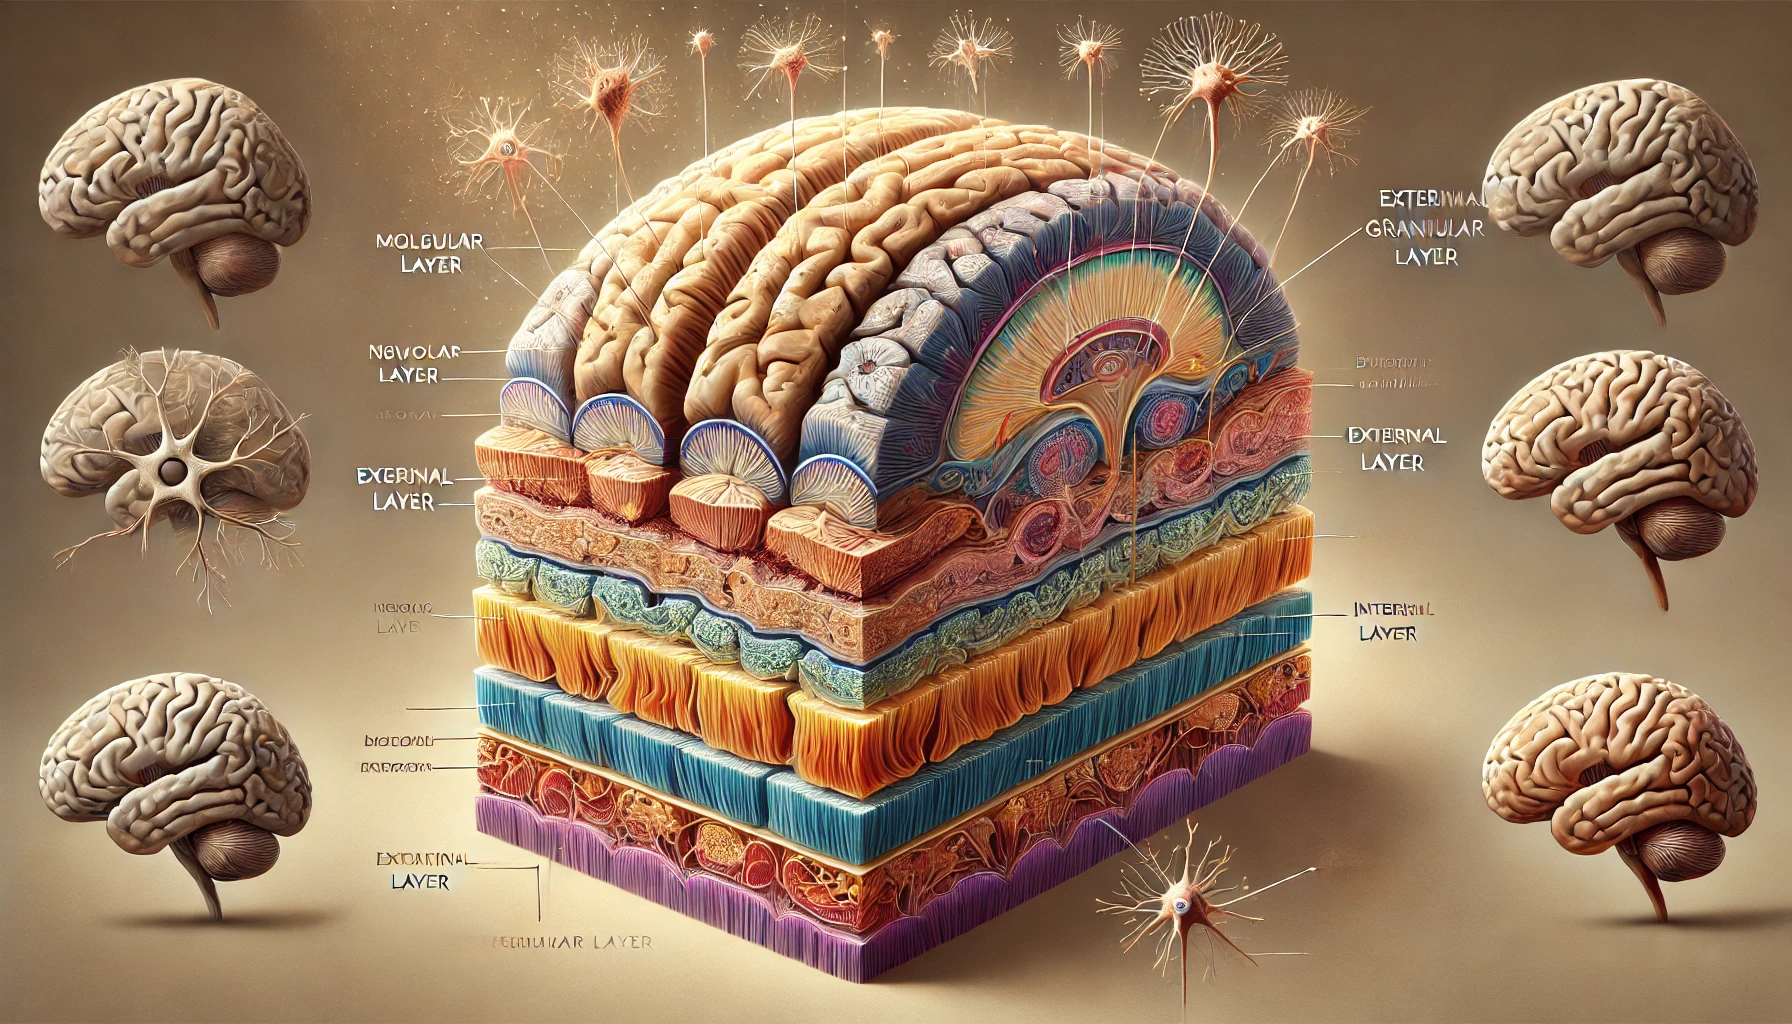
\includegraphics[width=0.8\textwidth]{cortical_layers.png}

    \caption{Cortical layers}
\end{figure}

The neuropil's dense connectivity serves multiple critical functions in maintaining conscious states \cite{Kasthuri2015}. Through its precise spatial organization, it enables coordinated interactions between neurons and glia while providing structured pathways for field-like effects to propagate. The arrangement of cellular processes creates an intricate three-dimensional matrix that supports both local processing and global integration of neural activity.

Astrocytic processes within the neuropil form an essential component of this architecture \cite{Peters1984}. Their elaborate branching patterns and strategic positioning allow them to monitor and modulate synaptic activity while maintaining ion homeostasis across substantial volumes of neural tissue. This spatial organization enables astrocytes to coordinate energy distribution and maintain coherent states across multiple spatial scales.

The extracellular matrix embedded within the neuropil provides another crucial architectural element \cite{Braitenberg1998}. Its molecular scaffolding helps stabilize synaptic connections while influencing the diffusion of neurotransmitters and ions. The precise composition and organization of the matrix varies across brain regions, creating specialized microenvironments that support different aspects of neural processing and energy management.

Dendritic architecture within the neuropil deserves particular attention \cite{Rockland2020}. The intricate branching patterns of dendrites create overlapping fields of integration that allow neurons to sample inputs from diverse sources while maintaining specific computational properties. This architectural feature enables sophisticated information processing while supporting the establishment of coherent energy states across neural populations.

The spatial arrangement of synaptic connections within the neuropil reflects both specific computational requirements and energy efficiency constraints \cite{Markram2015}. Synapses cluster in patterns that minimize wiring length while maximizing information transfer, creating local processing units that can maintain stable energy states while remaining dynamically responsive to changing inputs. This organization supports the emergence of coherent activity patterns while enabling flexible reconfiguration based on computational demands.

Gap junctions between cells provide another essential architectural feature within the neuropil \cite{Zeng2017}. These direct cellular connections create alternative pathways for signal propagation and state sharing, enabling rapid synchronization of cellular assemblies without requiring synaptic transmission. The distribution and regulation of gap junctions helps establish domains of coordinated activity that can maintain coherent states across multiple spatial scales.

The integration of these various architectural elements - astrocytic processes, extracellular matrix, dendritic fields, synaptic clusters, and gap junctions - creates a physical substrate capable of supporting the sophisticated energy dynamics required for conscious processing \cite{Bassett2017}. This multi-scale organization enables both local specialization and global integration while maintaining the energetic efficiency necessary for sustained conscious activity.

Through this architectural organization, the brain achieves a remarkable balance between stability and flexibility \cite{Buzsaki2006}. The structured pathways for energy flow and information processing allow for the maintenance of coherent states while enabling dynamic responses to changing conditions. This sophisticated architecture, refined through evolution, provides the physical foundation necessary for consciousness to emerge from organized energy flows within neural tissue.

The architectural organization of neural tissue culminates in a system that supports multiple modes of information transmission and energy propagation \cite{VanEssen2018}. Beyond classical synaptic transmission, the neuropil's structure enables ephaptic coupling, volume transmission, and field effects that contribute to conscious processing. These various mechanisms operate simultaneously across different spatial and temporal scales, creating a rich landscape of possible interactions that support coherent conscious states.

The evolutionary refinement of this architecture reflects a delicate balance between competing demands \cite{Hilgetag2020}. The need for efficient information processing must be weighed against energy constraints, while requirements for stability must accommodate the need for plasticity and adaptation. The resulting structure represents a sophisticated solution to these competing pressures, enabling conscious processing through carefully organized patterns of energy flow.

Perhaps most remarkably, this neural architecture creates conditions for emergent properties that transcend the capabilities of individual components \cite{vonBartheld2016}. Through its precise organization across multiple scales, from molecular arrangements to global connectivity patterns, the brain's structure enables the emergence of conscious experience from coherent energy dynamics. This emergence depends not just on the properties of individual elements but on their precise spatial arrangement and coordinated interaction.

Understanding neural architecture through the lens of ECC provides crucial insights into both the possibilities and constraints of conscious processing. The physical structure of neural tissue determines what patterns of energetic coherence can be maintained, what forms of information processing are possible, and what limitations must be respected. This architectural foundation proves essential for any complete theory of consciousness.

\section{Brain Waves}

Building on the neural architecture's structural foundation, brain waves emerge as primary mechanisms for implementing ECC's principles of state sharing and coherence maintenance. These oscillatory patterns, propagating through the neuropil's structured pathways, enable energetic coherence through tightly coupled state sharing across cortical regions \cite{Buzsaki2004}. Unlike digital computers with their discrete state transitions, brain waves support continuous, field-like properties that better align with ECC's emphasis on coherent energy flows and dynamic stability.

Different frequency bands serve complementary functions in maintaining conscious coherence \cite{Wang2010}. Gamma oscillations enable precise local synchronization, creating tight coupling between adjacent neural populations. Beta rhythms facilitate intermediate-range coordination between functional areas, while alpha waves help regulate larger-scale integration and inhibition. Theta oscillations support memory integration and emotional processing, and delta rhythms contribute to global state regulation \cite{Steriade2006}. These frequency bands do not operate in isolation but form nested hierarchies of coordination, where higher-frequency local oscillations become phase-locked to slower rhythms, creating cross-frequency coherence that enables integration across different spatial and temporal scales \cite{Canolty2010}.

The neuropil's architecture supports wave propagation through several sophisticated mechanisms \cite{Buzsaki2006}. Local circuit organization creates resonant structures that can sustain oscillatory patterns, while gap junctions between interneurons enable rapid synchronization of local populations. Astrocytic networks modulate wave propagation and help maintain stability, and the extracellular matrix provides a structured medium that shapes wave dynamics. These mechanisms work together to create and maintain patterns of coherent activity essential for conscious processing.

Brain waves serve multiple crucial functions in implementing ECC's principles \cite{Varela2001}. They enable efficient distribution of information across regions while supporting the maintenance of coherent states through oscillatory synchronization. Through careful management of energy flows, waves provide an efficient mechanism for coordinating activity across distributed neural populations. Different frequency bands help define functional boundaries between conscious states while enabling smooth transitions between them.

The interaction between brain waves and the neuropil's architecture creates coherence fields - stable patterns of energy flow that support conscious processing while maintaining thermodynamic efficiency \cite{Fries2015}. These fields provide the physical basis for the mathematical structures described in ECC's formal framework, enabling both local processing and global integration through continuous, field-like interactions.

Perhaps most remarkably, brain waves demonstrate how neural systems can maintain coherent states while enabling dynamic reorganization \cite{Engel2001}. During transitions between conscious states, wave patterns shift in coordinated ways that preserve overall coherence while allowing for rapid reconfiguration of neural activity. This capacity for stable yet flexible organization proves essential for maintaining conscious experience in the face of constantly changing environmental demands.

The coordination between brain waves and astrocytic networks deserves particular attention. While neurons generate the primary oscillatory patterns, the stability and propagation of these waves rely heavily on the regulatory influence of astrocytes \cite{Ward2003}. Brain waves propagating through the neuropil interact continuously with astrocytic networks, which help maintain proper conditions for coherent activity by regulating ion concentrations in the extracellular space, modulating synaptic transmission, coordinating metabolic support, and buffering excessive activity.

This sophisticated interaction between neuronal oscillations and glial regulation creates the conditions necessary for maintaining coherent conscious states while enabling dynamic responses to changing conditions \cite{Basar2013}. The resulting system demonstrates how biological organization can achieve both stability and flexibility through carefully orchestrated patterns of energy flow.

The relationship between brain waves and conscious experience reveals itself through multiple complementary mechanisms \cite{Jensen2007}. Oscillatory patterns create temporal windows for information integration, enabling distributed neural populations to coordinate their activity with precise timing. These windows of synchronization allow for the binding of sensory inputs, the coordination of motor outputs, and the integration of internal states into coherent conscious experiences.

The hierarchical organization of brain waves proves particularly significant for consciousness \cite{Lisman2013}. Slower oscillations modulate the amplitude of faster rhythms, creating nested patterns of activity that support both local processing and global integration. This cross-frequency coupling enables the brain to maintain multiple simultaneous processes while preserving overall coherence. For instance, theta rhythms may organize sequences of gamma-band activity, creating structured packages of information processing that can be integrated into broader conscious experiences.

Wave propagation through neural tissue demonstrates remarkable sophistication in managing energy distribution \cite{Palva2012}. Rather than broadcasting signals indiscriminately, brain waves follow specific paths shaped by the underlying neural architecture. These paths, established through both structural and functional connectivity, enable efficient communication between distributed regions while minimizing energy expenditure. The resulting patterns of activity support both the specificity required for precise information processing and the broader coordination necessary for conscious integration.

State transitions in consciousness correlate strongly with shifts in oscillatory patterns \cite{Singer2018}. During changes in attention, alertness, or cognitive focus, brain waves reorganize in coordinated ways that maintain overall stability while enabling adaptive responses to new demands. These transitions demonstrate how neural systems can achieve both continuity and flexibility through careful orchestration of oscillatory dynamics. The ability to maintain coherent states while enabling rapid reconfiguration proves essential for conscious processing.

The interaction between brain waves and metabolic processes reveals another layer of sophistication \cite{Nyhus2010}. Oscillatory patterns help coordinate energy delivery to active neural populations, ensuring that metabolic resources are distributed efficiently according to computational demands. This coupling between neural activity and energy metabolism, mediated in part through astrocytic networks, helps maintain the precise balance of excitation and inhibition necessary for conscious processing.

Beyond traditional synaptic and gap junction communication, ephaptic coupling - where neurons influence each other through local electric fields - plays a crucial role in wave propagation \cite{Buzsaki2006}. These field effects enable rapid coordination across neural populations without requiring direct anatomical connections. The resulting electromagnetic interactions contribute to the formation and maintenance of coherent oscillatory states, particularly in densely packed neural tissue where field effects become more prominent.

Pathological conditions affecting consciousness often manifest as disruptions in normal oscillatory patterns \cite{Uhlhaas2010}. Whether through trauma, disease, or pharmaceutical intervention, alterations in brain wave dynamics frequently correspond to changes in conscious experience. These correlations provide valuable evidence for the essential role of coherent oscillatory activity in maintaining conscious states.

Research on anesthesia further illuminates the relationship between brain waves and consciousness \cite{Kahana2001}. Different anesthetic agents produce characteristic changes in oscillatory patterns that correlate with the loss and recovery of consciousness. These effects suggest that proper orchestration of brain waves is not merely correlated with but causally necessary for conscious experience.

The complex interplay between brain waves, metabolic demands, and neural architecture culminates in a system capable of maintaining conscious states across multiple temporal and spatial scales \cite{Varela2001}. Through carefully orchestrated oscillatory patterns, the brain achieves a remarkable balance between stability and adaptability, enabling coherent conscious experience while remaining responsive to changing environmental demands and internal needs.

These oscillatory dynamics provide crucial insights into both the mechanisms and limitations of consciousness. The specific frequency bands, their interactions, and the physical constraints on their propagation help explain why conscious processing exhibits particular temporal and spatial boundaries. Understanding these constraints proves essential for any complete theory of how consciousness emerges from neural activity.

Perhaps most significantly, brain waves demonstrate how biological systems can achieve sophisticated information processing through continuous, field-like properties rather than discrete computational steps \cite{Singer2018}. This insight aligns with ECC's broader emphasis on consciousness as emerging from coherent energy dynamics rather than abstract symbol manipulation. The resulting framework suggests new approaches to understanding both biological consciousness and the potential development of artificial conscious-like systems.

\section{Astrocytic Networks}

The astrocytic contribution to conscious processing extends far beyond mere metabolic support of neuronal activity. Astrocytes form extensive networks through gap junctions, creating syncytia that span significant portions of neural tissue \cite{Giaume2010}. These syncytial networks serve as a parallel processing system that operates on slower timescales than neuronal circuits but provides crucial mechanisms for maintaining coherent conscious states.

Unlike neurons, which communicate primarily through discrete synaptic events, astrocytic syncytia enable direct cytoplasmic continuity between cells, allowing for seamless sharing of ions, metabolites, and signaling molecules across extended spatial domains \cite{Nagy2000}. This continuous internal medium creates an ideal substrate for maintaining coherent energy states over longer timescales than typical neuronal interactions.

The astrocytic networks demonstrate remarkable sophistication in their spatial organization \cite{Oberheim2012}. These networks can span multiple cortical columns, creating continuous domains for ion and metabolite distribution that transcend traditional anatomical boundaries. Through this extensive connectivity, astrocytic syncytia enable coordination across broader spatial domains than possible through neuronal connections alone, while providing mechanisms for stabilizing coherent energy states across neural tissue.

Temporal integration through astrocytic networks occurs on a fundamentally different scale than neuronal processing \cite{Bazargani2016}. Operating on timescales of seconds rather than milliseconds, astrocytes generate calcium waves that propagate across the syncytial network, maintaining stable background states that help regulate neuronal activity. This slower processing provides a complementary mechanism to rapid neuronal signaling, enabling the maintenance of coherent states across longer temporal windows.

The metabolic regulation provided by astrocytic networks proves essential for conscious processing \cite{Verkhratsky2018}. These networks coordinate energy distribution across active neural populations, maintain ion homeostasis in the extracellular space, and regulate neurotransmitter levels at synapses. Through these mechanisms, astrocytic syncytia support efficient energy utilization while enabling sustained conscious processing across distributed neural populations.

The interaction between astrocytic networks and neuronal systems creates a multi-scale organization where fast neuronal signaling becomes embedded within slower, more stable astrocytic domains \cite{Halassa2010}. This arrangement provides several crucial advantages for maintaining conscious states. The slower astrocytic processes help maintain coherent background states, while the syncytial networks enable coordination across extended spatial domains. Direct sharing of resources through the syncytial network supports sustained activity, while the combination of fast neuronal and slow astrocytic processes enables dynamic yet stable conscious states.

\begin{figure}[h]
    \centering
    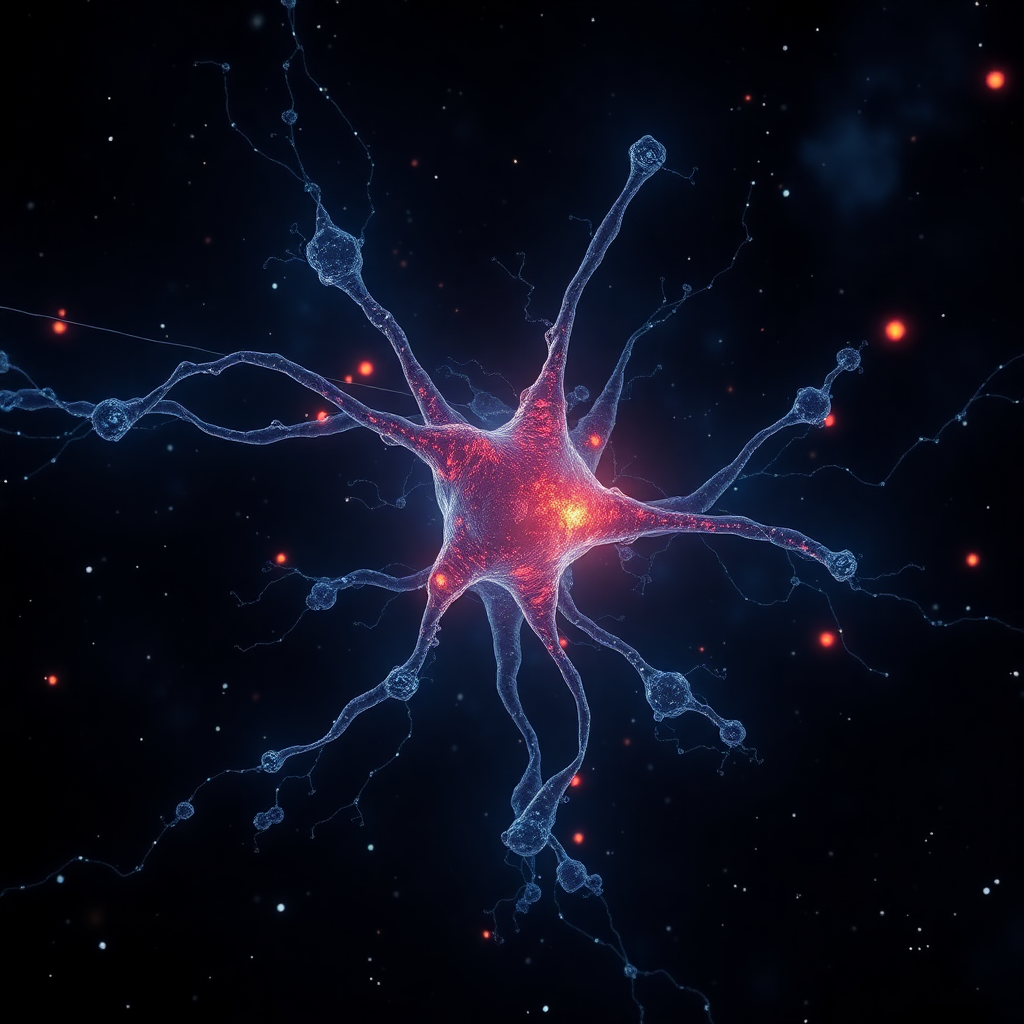
\includegraphics[width=0.8\textwidth]{images/astrocyte.png}

    \caption{Typical astrocyte.}
\end{figure}

The remarkable capacity of astrocytic networks to maintain coherent states while enabling dynamic responses becomes particularly evident in their role as regulators of neural excitability. Through careful modulation of extracellular ion concentrations and neurotransmitter levels, astrocytes help establish the precise conditions necessary for stable neural processing \cite{Araque2014}. This regulatory function extends beyond simple homeostasis to include active participation in information processing and state transitions.

Calcium signaling within astrocytic networks deserves particular attention \cite{Bazargani2016}. Unlike the rapid electrical signaling of neurons, astrocytes communicate through complex patterns of calcium waves that propagate across the syncytial network. These calcium signals can integrate information over longer temporal windows than neuronal activity, providing a mechanism for maintaining coherent states across extended periods. The patterns of calcium wave propagation reflect both local neural activity and broader network states, creating a sophisticated system for coordinating neural responses across multiple spatial and temporal scales.

The relationship between astrocytic networks and brain waves reveals another crucial aspect of conscious processing. Astrocytes help establish the conditions necessary for coherent oscillatory activity while modulating the spread of these oscillations through neural tissue \cite{Volterra2005}. Through regulation of extracellular ion concentrations and neurotransmitter dynamics, astrocytic networks can influence both the generation and propagation of brain waves. This interaction creates a feedback system where neuronal oscillations and astrocytic signaling work together to maintain stable patterns of conscious activity.

Gap junctions between astrocytes play an essential role in establishing the syncytial properties that enable coherent state maintenance \cite{Wallraff2006}. These direct cellular connections allow for rapid sharing of ions, metabolites, and small signaling molecules across extended spatial domains. The density and distribution of gap junctions can be dynamically regulated, providing a mechanism for modulating the extent and strength of network coupling based on current physiological demands.

The relationship between astrocytic networks and neural metabolism reveals sophisticated mechanisms for maintaining conscious states \cite{Parpura2012}. Through their extensive processes, astrocytes form specialized contacts with both blood vessels and synapses, creating a distributed system for matching energy supply to neural demand. This arrangement enables precise control over local metabolic conditions while maintaining broader patterns of energy distribution across neural tissue.

The integration of astrocytic networks with other brain systems demonstrates how biological organization can achieve both stability and flexibility through coordinated cellular interactions \cite{Khakh2015}. The ability of astrocytes to monitor and modulate neural activity while maintaining coherent energy states across extended spatial domains provides essential mechanisms for conscious processing. This sophisticated arrangement allows the brain to maintain stable conscious states while remaining adaptable to changing environmental demands.

Perhaps most significantly, astrocytic networks demonstrate how consciousness emerges not from neuronal activity alone but from the coordinated interaction of multiple cellular systems \cite{Nedergaard2003}. The continuous, field-like properties of astrocytic syncytia complement the discrete signaling of neurons, creating a hybrid system capable of supporting both rapid information processing and stable state maintenance. This integration of different cellular mechanisms proves essential for understanding how conscious states arise from biological organization.

The remarkable efficiency of astrocytic networks in managing ion homeostasis illustrates fundamental principles of conscious processing \cite{Bellot-Saez2017}. Through sophisticated regulation of extracellular potassium and calcium levels, these networks maintain the precise ionic conditions necessary for reliable neural signaling while preventing pathological states of over-excitation. This homeostatic function represents more than simple buffering - it creates the stable background conditions required for coherent conscious processing.

The study of astrocytic networks thus reveals fundamental principles about how biological systems achieve conscious processing \cite{Giaume2010}. Through their unique properties and extensive connectivity, astrocytes help create the conditions necessary for consciousness while providing mechanisms for maintaining coherent states across multiple spatial and temporal scales. This understanding proves essential for any complete theory of consciousness and suggests new approaches to both treating disorders of consciousness and developing artificial conscious-like systems.

The implications extend beyond neuroscience to fundamental questions about how biological systems maintain coherent states across multiple scales of organization \cite{Khakh2015}. The remarkable sophistication of gap junction networks demonstrates how evolution has refined cellular coupling mechanisms to support both stable conscious states and flexible adaptation to changing conditions. This deeper appreciation of biological connectivity proves essential for any complete theory of consciousness.

Moving beyond cellular networks, we must now examine how the extracellular matrix provides crucial structural and functional support for conscious processing. This complex network of proteins and molecules outside cells creates specialized microenvironments that shape both energy flows and information processing in neural tissue.

\section{The Extracellular Matrix}

The extracellular matrix serves as more than just structural scaffolding for neural tissue. It forms an active component of the brain's information processing and energy management systems \cite{Dityatev2010}. This complex network of proteins, proteoglycans, and other molecules fills the space between cells, creating a structured environment that shapes both ionic flows and molecular signaling while providing crucial support for maintaining coherent states.

The interaction between astrocytic networks and the ECM proves particularly important for maintaining energetic coherence across subsystems \cite{Song2018}. The ECM creates organized diffusion pathways that guide the movement of ions and neurotransmitters through the extracellular space, helping regulate local signaling environments while supporting broader patterns of communication across neural tissue. This structured diffusion plays an essential role in shaping both synaptic transmission and volume transmission between cells \cite{Sykova2008}.

The molecular composition and organization of the ECM varies systematically across brain regions, reflecting local functional requirements and computational demands \cite{Bandtlow2000}. These regional specializations create distinct microenvironments that support different aspects of neural processing. Through specific arrangements of matrix proteins and proteoglycans, the ECM helps establish and maintain the precise conditions necessary for different forms of neural computation and state maintenance \cite{Zimmermann2008}.

Perineuronal nets, specialized ECM structures that surround specific neuronal subtypes, demonstrate particularly sophisticated organization \cite{Wang2012}. These nets stabilize synaptic connections while regulating local ion concentrations, enabling sustained high-frequency firing patterns in certain neural populations. The precise molecular composition of perineuronal nets helps create stable microenvironments that support reliable neural signaling while allowing for controlled plasticity \cite{Kwok2011}.

The broader interstitial matrix that fills the space between cells serves multiple crucial functions in neural processing \cite{Ruoslahti1996}. Beyond providing structural support, this matrix guides molecular diffusion, supports volume transmission, and helps maintain proper spacing between cellular elements \cite{Nicholson1998}. The physical properties of the interstitial matrix influence both local signaling dynamics and broader patterns of communication across neural tissue.

The dynamic interaction between cellular components and the ECM creates a structured environment that supports both stability and adaptability in neural processing \cite{Dityatev2003}. Rather than serving as a static scaffold, the ECM actively participates in shaping neural activity through its influence on molecular diffusion, ion distribution, and cellular communication. This dynamic role proves essential for maintaining the coherent states necessary for conscious processing.

\begin{figure}[h]
    \centering
    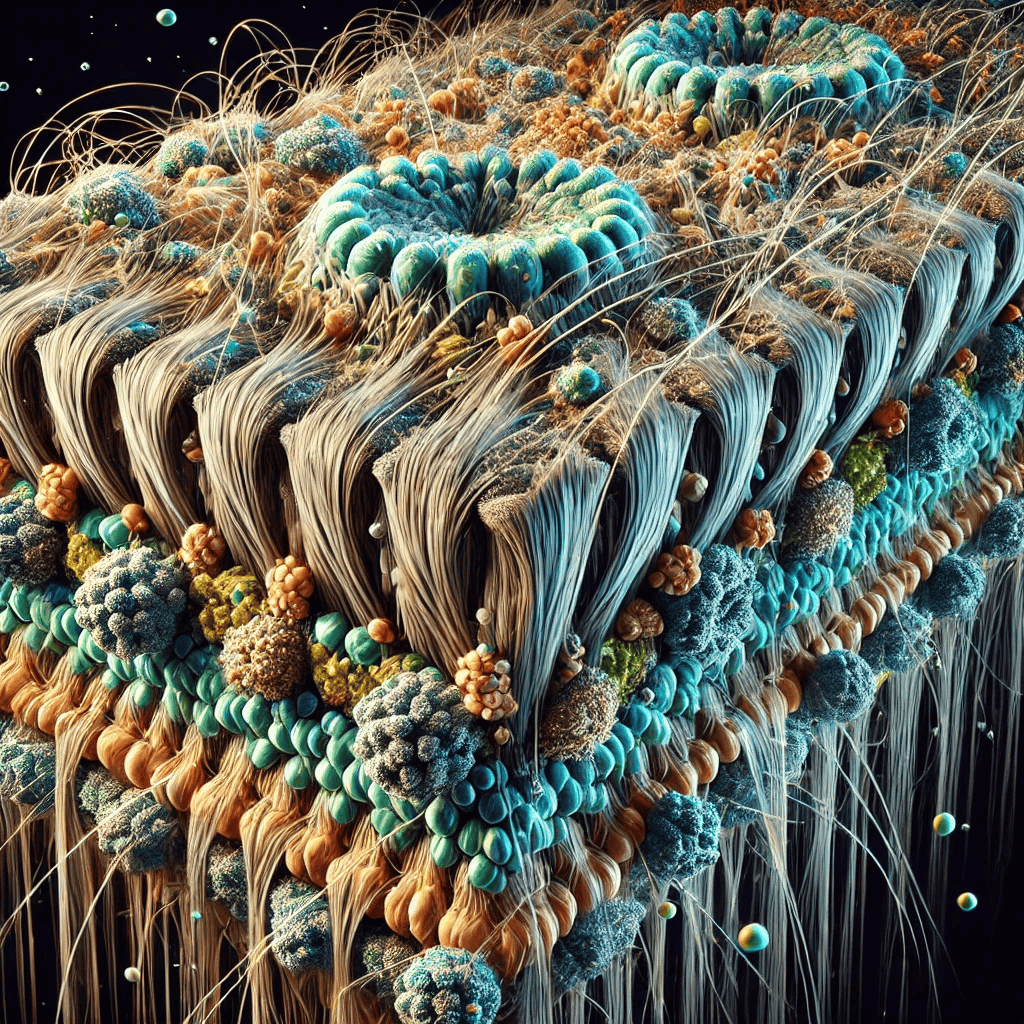
\includegraphics[width=0.8\textwidth]{ecm.png}

    \caption{The ECM guides ion flows and EM waves.}
\end{figure}

The ECM's influence on neural signaling extends beyond traditional synaptic transmission \cite{Vargova2014}. Through its capacity to bind and concentrate various signaling molecules, the matrix creates specialized signaling domains that shape both local and long-range communication. These domains help orchestrate complex patterns of neural activity while maintaining the stability necessary for coherent processing. The matrix's ability to sequester and release molecules in response to neural activity provides an additional layer of regulation in neural computation.

The relationship between the ECM and neural plasticity reveals sophisticated mechanisms for balancing stability and adaptability \cite{Dityatev2010}. While perineuronal nets help stabilize existing synaptic connections, local modifications of matrix composition can enable controlled reorganization of neural circuits \cite{Burnside2014}. This dynamic regulation of plasticity proves essential for learning and memory while maintaining the overall stability necessary for conscious processing.

Water and ion movement through the extracellular space depends critically on ECM organization \cite{Hrabetova2009}. The matrix creates structured pathways that guide fluid flow and ion diffusion, influencing both local signaling dynamics and broader patterns of neural activity. These pathways help maintain proper ionic balance while enabling efficient distribution of metabolites and removal of waste products. The resulting flow patterns support both local computation and global integration of neural activity.

The ECM's role in maintaining boundary conditions between different neural compartments deserves particular attention \cite{Barros2011}. Through specific molecular arrangements, the matrix helps establish and maintain distinct functional domains within neural tissue. These boundaries prove essential for proper circuit function while enabling controlled communication between different neural populations \cite{Frischknecht2012}. The precise organization of these boundary regions reflects evolutionary optimization for both isolation and integration of neural processing.

Matrix metalloproteinases and other ECM-modifying enzymes provide mechanisms for dynamic regulation of extracellular space properties \cite{Dityatev2003}. These enzymes can rapidly modify local matrix composition in response to neural activity, enabling adaptive changes in diffusion properties and signaling environments. This dynamic regulation allows neural circuits to adjust their processing capabilities while maintaining overall stability \cite{Song2018}.

The interaction between the ECM and glial cells represents another crucial aspect of neural organization \cite{Vargova2014}. Astrocytes actively participate in maintaining and modifying matrix composition, creating a feedback system that enables dynamic regulation of extracellular space properties. This interaction helps coordinate local changes in matrix structure with broader patterns of neural activity and metabolic demand.

The ECM's contribution to energetic coherence becomes particularly evident in its role in maintaining field effects across neural tissue \cite{Sykova2008}. The structured organization of matrix molecules influences the propagation of electromagnetic fields generated by neural activity, helping shape both local and global patterns of field interaction. This influence on field dynamics provides another mechanism through which the matrix contributes to conscious processing.

Understanding the ECM through ECC's framework reveals how seemingly passive structural elements can play active roles in consciousness \cite{Dityatev2010}. The matrix emerges not merely as a support system but as an essential component in maintaining the coherent energy states necessary for conscious experience. Its sophisticated molecular organization and dynamic properties enable both the stability required for reliable neural processing and the flexibility needed for adaptive responses \cite{Frischknecht2012}.

This deeper appreciation of the ECM's role suggests new approaches to both understanding and treating disorders of consciousness \cite{Burnside2014}. Matrix disruptions may contribute to various pathological conditions through their effects on neural signaling and energy coherence. Conversely, therapeutic interventions targeting matrix composition or organization might provide novel ways to influence conscious states and restore normal brain function.

The ECM's role extends beyond local circuit function to influence global brain dynamics \cite{Barros2011}. Through its effects on ion mobility, volume transmission, and field propagation, the matrix helps establish the conditions necessary for maintaining coherent states across multiple spatial scales. This multi-scale organization proves essential for understanding how consciousness emerges from coordinated neural activity \cite{Zimmermann2008}.

Having examined the biological components of neural tissue, we must now consider how to model the complex interactions within the neuropil that give rise to conscious states. This dense network of neural processes, glial cells, and extracellular matrix presents unique challenges for mathematical description and computational simulation.

\section{Neuropil Modeling}

The neuropil represents the brain's primary substrate for maintaining coherent conscious states, integrating cellular networks, ECM, and interstitial space into a unified functional domain. This dense meshwork of neural processes (including dendrites and their spines), glial elements, and extracellular structures creates an ideal medium for supporting organized energy flows and information integration \cite{Kasthuri2015}.

\begin{figure}[h]
    \centering
    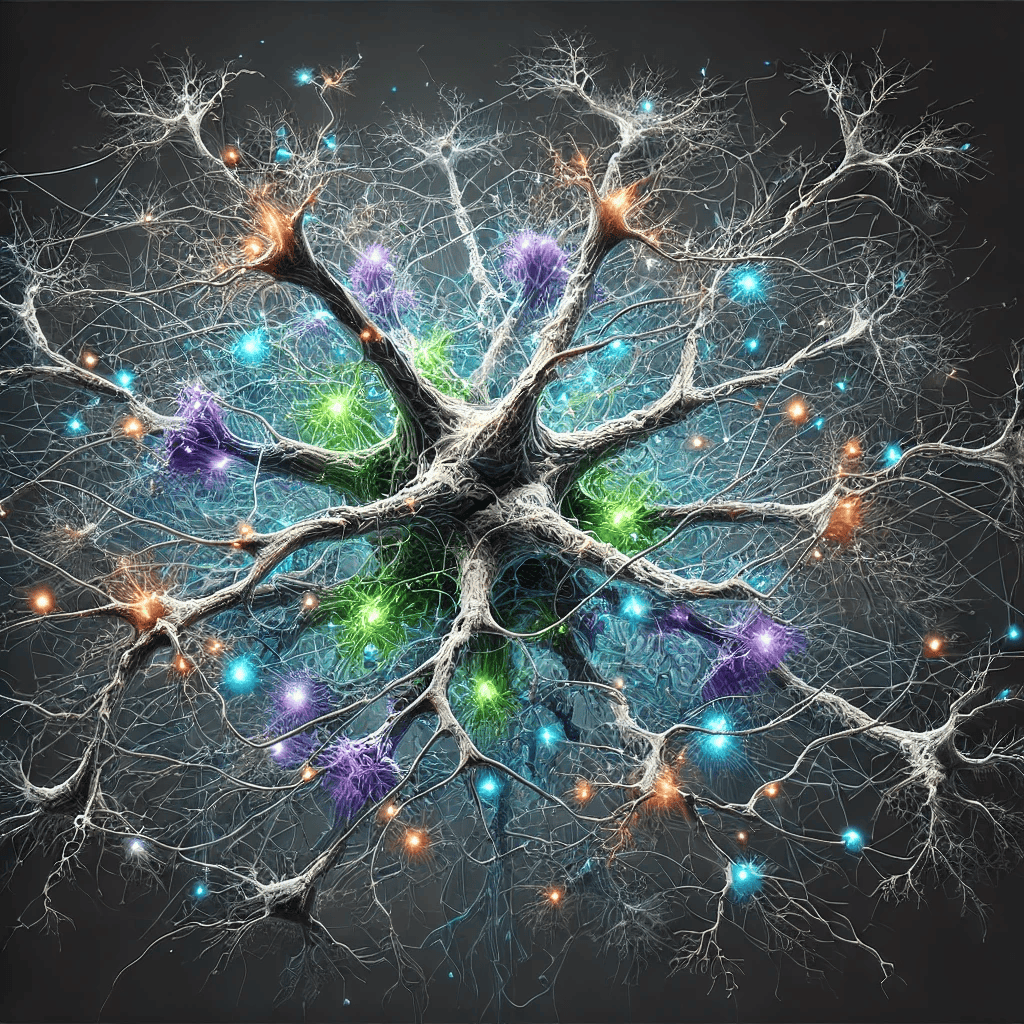
\includegraphics[width=0.8\textwidth]{neuropil.png}

    \caption{The neuropil is the most tangled layer of the cortical sheet}
\end{figure}

To model energetic coherence in the neuropil, we can employ the Jacobian of the stress-energy tensor with specific coupling terms that capture interactions between different components:

$\partial_\sigma T_{\mu\nu}(x) = \sum_i J_i(x) + \sum_{j,k} C_{jk}(x)$

\text{Where:}
\begin{itemize}
\item $T_{\mu\nu}$ represents the stress-energy tensor for the neuropil
\item $J_i$ captures local energy flows within specific components
\item $C_{jk}$ represents coupling terms between different elements
\item $x$ denotes position within the neuropil space
\end{itemize}

This organization creates the conditions necessary for sustained coherent states through the precise balance of energy flows across multiple scales \cite{Mishchenko2010}. When we examine the temporal evolution of these states, we can represent the dynamics using a modified form of the stress-energy tensor's Jacobian that incorporates both spatial and temporal derivatives:

$\partial_\sigma\partial_\tau T_{\mu\nu} = \sum_i \partial_\sigma J_i + \sum_{j,k} \partial_\tau C_{jk} + I_{\mu\nu}$

\text{Where:}
\begin{itemize}
\item $\partial_\sigma\partial_\tau$ represents the spatiotemporal evolution
\item $I_{\mu\nu}$ captures interface terms between adjacent regions
\end{itemize}

The interface terms are particularly important for understanding how coherent states propagate through the neuropil \cite{Doron2017}. These terms must satisfy certain continuity conditions:

$I_{\mu\nu}|_{\text{boundary}} = \text{continuous across regions}$

This constraint ensures smooth transitions between adjacent domains while maintaining global coherence. The neuropil's structure supports these transitions through specific biophysical mechanisms and architectural organization \cite{Korogod2015}.

1. Local Field Dynamics:

$\nabla \cdot \mathbf{E} = \frac{\rho}{\varepsilon}$

\text{Where:}
\begin{itemize}
\item $\mathbf{E}$ represents local field strength
\item $\rho$ captures charge density
\item $\varepsilon$ reflects local permittivity \cite{Savtchenko2014}
\end{itemize}

2. Wave Propagation:

$(\nabla^2 - \frac{1}{v^2}\frac{\partial^2}{\partial t^2})\psi = 0$

\text{Where:}
\begin{itemize}
\item $\psi$ represents the wave function
\item $v$ is the propagation velocity in the medium \cite{Arbib1998}
\end{itemize}

These equations describe how the neuropil supports both standing waves and propagating disturbances while maintaining coherent states. The solution space is constrained by the physical properties of the neuropil \cite{Peters1991}.

These constraints help ensure that energy flows remain within bounds that support conscious processing while allowing for dynamic responses to changing conditions \cite{Sorra2000}. The neuropil thus emerges as the critical substrate for implementing ECC's principles, providing both the physical structure and dynamic properties necessary for maintaining coherent conscious states.

\begin{figure}[h]
    \centering
    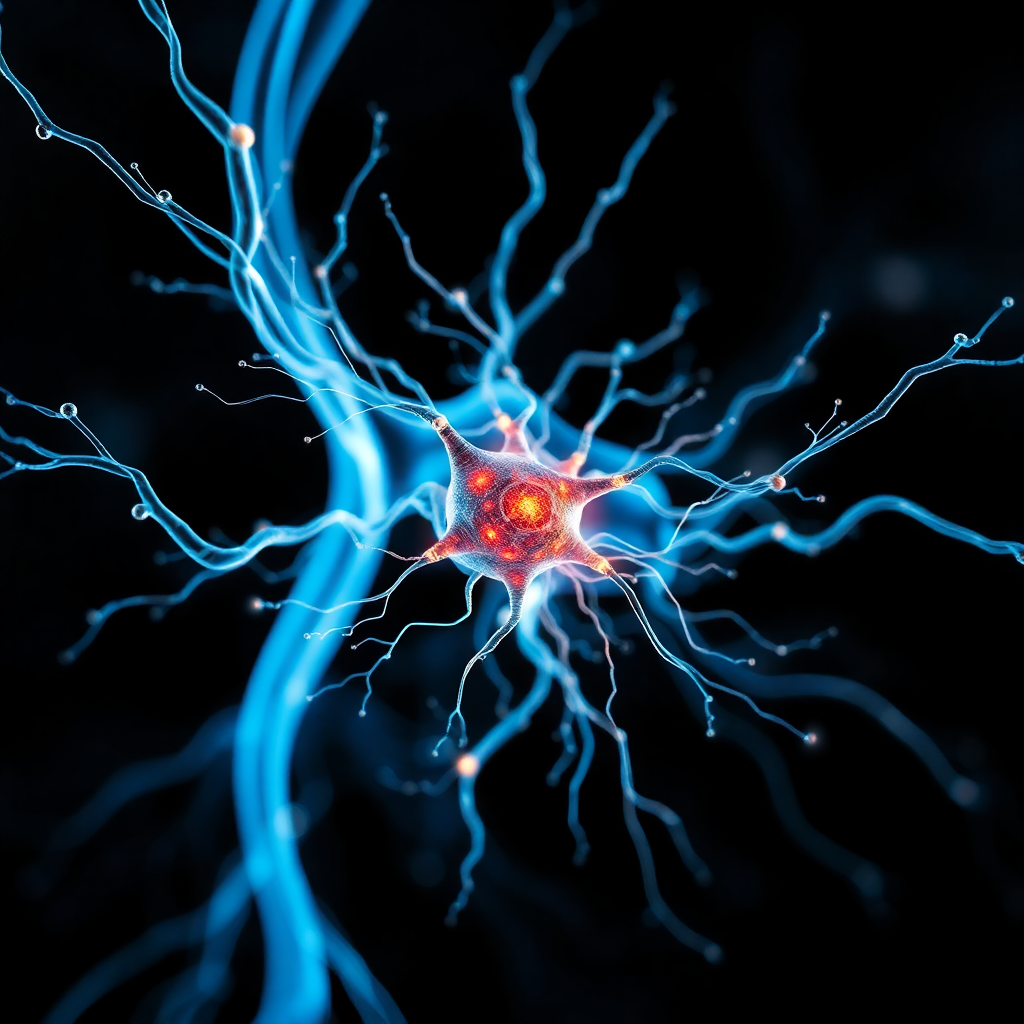
\includegraphics[width=0.8\textwidth]{images/neuropil2.png}

    \caption{Typical neuron of the neuropil.}
\end{figure}

The neuropil represents a critical domain for understanding how conscious states emerge from neural organization, as it provides the physical substrate where energetic coherence manifests at multiple scales \cite{Ventura1999}. This dense mesh of neural processes, glial extensions, and extracellular matrix creates the conditions necessary for maintaining coherent energy states while enabling dynamic information processing. Understanding how these components interact within the neuropil proves essential for any complete theory of consciousness.

The significance of neuropil organization extends beyond traditional connectionist approaches that focus primarily on synaptic connections between neurons \cite{Kasthuri2015}. Within this intricate space, multiple modes of communication operate simultaneously, including volume transmission, ephaptic coupling, and field effects that influence neural activity through non-synaptic mechanisms. These various forms of interaction create a rich landscape of possible states that supports both local processing and global integration of neural activity.

The physical properties of the neuropil prove particularly crucial for maintaining energetic coherence \cite{Korogod2015}. Its precise spatial organization enables the establishment of stable field patterns while allowing for rapid reconfiguration based on computational demands. The density and arrangement of cellular processes within the neuropil create conditions that support wave propagation while maintaining boundaries between different functional domains \cite{Arbib1998}. This balanced organization enables both segregation and integration of neural processing.

Astrocytic processes within the neuropil play an especially important role in maintaining coherent states \cite{Ventura1999}. Their extensive branching patterns and strategic positioning allow them to monitor and modulate synaptic activity while maintaining ion homeostasis across substantial volumes of tissue. The three-dimensional organization of astrocytic processes creates a continuous network that can coordinate energy distribution and maintain stable background conditions necessary for conscious processing.

The extracellular space within the neuropil, far from being a simple gap between cells, represents a highly structured environment that shapes both molecular diffusion and field effects \cite{Savtchenko2014}. The precise arrangement of extracellular matrix components influences how signals propagate through this space, affecting both local interactions and longer-range coordination. This structured environment proves essential for maintaining the specific patterns of energy flow that support conscious states.

The dynamic nature of neuropil organization deserves particular attention \cite{Sorra2000}. Rather than representing a static structure, the neuropil continuously adapts its properties in response to neural activity and metabolic demands. This adaptability enables sophisticated regulation of energy distribution and information processing while maintaining the stability necessary for coherent conscious experience. Understanding these dynamics proves crucial for developing accurate models of how consciousness emerges from neural activity.

Moreover, the neuropil's organization reflects evolutionary optimization for both information processing efficiency and energy management \cite{Peters1991}. The precise arrangement of cellular processes minimizes wiring length while maximizing computational capacity, creating conditions that support conscious processing while respecting metabolic constraints. This efficiency proves essential for maintaining coherent states across extended periods without excessive energy expenditure.

These considerations reveal why detailed modeling of neuropil organization and dynamics proves essential for understanding consciousness \cite{Mishchenko2010}. The emergence of coherent conscious states depends critically on the specific properties and interactions that occur within this complex domain. Any complete theory of consciousness must account for how the neuropil's structure enables both local processing and global integration while maintaining energetic efficiency.

The challenge of modeling neuropil dynamics reflects deeper questions about how consciousness emerges from biological organization \cite{Denk2004}. Traditional computational approaches, focused primarily on discrete neuronal interactions, fail to capture the continuous, field-like properties that arise from the neuropil's intricate structure. New mathematical frameworks must be developed that can represent both the discrete and continuous aspects of neural processing while accounting for the multiple scales of organization present in neural tissue.

The integration of various modeling approaches becomes particularly crucial when considering the neuropil's role in conscious processing \cite{Haehn2014}. Field theories must be combined with detailed cellular models, while accounting for the structured diffusion processes that occur in the extracellular space. These different perspectives must be unified through mathematical frameworks that can capture both the local dynamics of individual components and the emergent properties that arise from their collective interaction.

Perhaps most significantly, neuropil modeling reveals fundamental principles about how biological systems achieve conscious processing \cite{Helmstaedter2013}. The sophisticated organization of the neuropil, with its multiple overlapping domains of interaction and regulation, demonstrates how complex conscious states can emerge from physical processes while maintaining both stability and adaptability. This understanding proves essential for both theoretical developments in consciousness studies and practical applications in treating neurological disorders.

The implications extend beyond neuroscience to influence our broader understanding of consciousness itself \cite{White1986}. The neuropil's organization suggests that consciousness requires specific forms of physical implementation that support both local processing and global integration through continuous field-like interactions. This perspective challenges purely computational approaches to consciousness while suggesting new directions for developing artificial systems that might support conscious-like processing.

\section{Brodmann Areas}

The functional organization of the cortex into distinct Brodmann areas reflects a deeper principle of regional specialization that extends beyond cytoarchitecture to the molecular level. Each Brodmann area possesses a unique transcriptomic profile - a specific pattern of gene expression that shapes its information processing capabilities and energy management strategies \cite{Amunts2015}. These molecular signatures help explain how different regions maintain distinct functional properties while participating in the broader field of conscious experience.

Unlike the traditional view of Brodmann areas as purely structural divisions, modern neuroscience reveals them as domains of specialized molecular organization \cite{Amunts2007}. Brodmann areas represent distinct regions of the cerebral cortex, first mapped by neuroanatomist Korbinian Brodmann in the early 20th century based on their unique cytoarchitectural organization \cite{Brodmann1909}. These areas differ in the thickness of cortical layers, density of neurons, types of cells present, and patterns of connectivity. Originally identified through careful microscopic examination of cell structure and arrangement, these regions have since been shown to correspond closely with functional specialization in the brain \cite{Eickhoff2018}.

Each Brodmann area exhibits characteristic properties that reflect its role in processing specific types of information. For example, primary visual cortex (Brodmann area 17) shows a prominent layer 4 that receives direct thalamic input, while motor cortex (Brodmann area 4) is characterized by large pyramidal neurons in layer 5 that project to the spinal cord \cite{Zilles2010}. These structural differences support each region's specialized function while maintaining the capacity to integrate into broader conscious processes.

The functional organization of the cortex into distinct regions, mapped through careful cytoarchitectural analysis, takes on profound new significance when examined through the framework of energetically coherent computation. Far from being merely anatomical subdivisions, these areas represent domains of specialized molecular organization that enable distinct patterns of energetic coherence while maintaining integration with broader conscious processes \cite{Glasser2016}.

Unlike the traditional view of Brodmann areas as purely structural divisions, modern neuroscience reveals them as domains of sophisticated molecular organization \cite{Hawrylycz2012}. Each area maintains unique transcriptomic profiles that shape its capacity for information processing and energy management. These molecular signatures help explain how different regions maintain distinct functional properties while participating in the broader field of conscious experience.

The cellular architecture of each Brodmann area reflects evolutionary optimization for specific forms of information processing \cite{Palomero-Gallagher2019}. Areas devoted to sensory processing, such as primary visual cortex, demonstrate precisely organized cellular arrangements that support rapid, parallel processing of sensory inputs. In contrast, association areas maintain more flexible architectures that enable complex integration of information from multiple sources. These structural differences support each region's specialized function while maintaining the capacity for integration into broader conscious processes.

\begin{figure}[h]
    \centering
    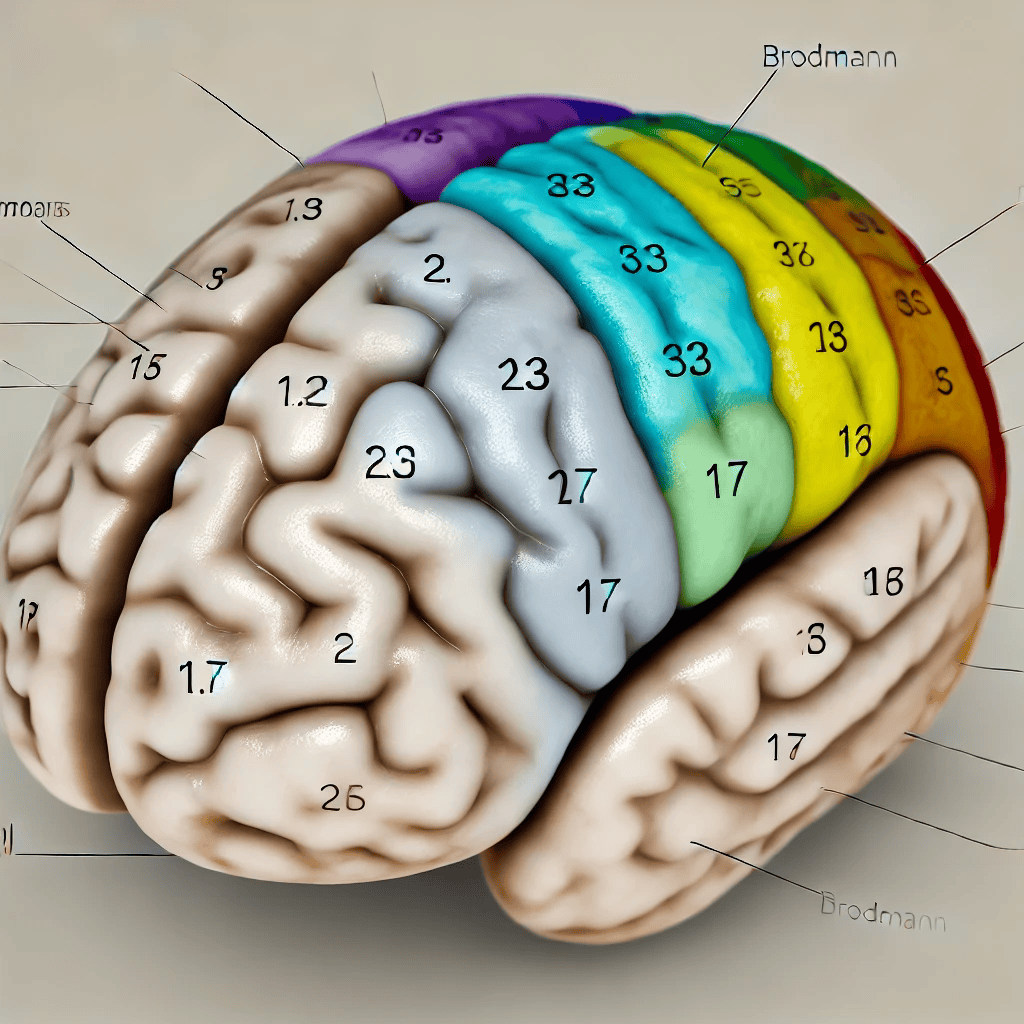
\includegraphics[width=0.8\textwidth]{brodmann.png}

    \caption{Brodmann areas align with great variation in transcriptomic profiles}
\end{figure}

The relationship between cellular organization and energetic coherence becomes particularly evident when examining how different Brodmann areas process information \cite{Passingham2002}. Primary sensory areas maintain tightly organized columns that enable precise mapping of sensory inputs while supporting stable patterns of energetic coherence. Association areas demonstrate more distributed patterns of organization that allow for flexible integration of information while maintaining coherent energy states across larger spatial domains.

Transcriptomic analysis reveals how each Brodmann area expresses distinct combinations of ion channels, receptors, and metabolic enzymes that shape its functional properties \cite{Lake2018}. These molecular profiles determine not just the computational capabilities of each region but also its capacity for maintaining specific patterns of energetic coherence. The resulting specialization enables sophisticated processing of different types of information while supporting integration into unified conscious experiences.

The patterns of connectivity between Brodmann areas reflect both computational requirements and energetic constraints \cite{VanEssen2012}. Long-range connections between regions must balance the need for efficient information transfer against the metabolic costs of maintaining extended axonal processes. This optimization creates networks that can support complex conscious processing while respecting fundamental energetic limitations.

The hierarchical organization of Brodmann areas reveals sophisticated principles of information processing and energy management \cite{Amunts2015}. Primary sensory areas maintain relatively rigid patterns of coherence that enable faithful representation of sensory inputs, while higher association areas demonstrate more flexible organizations that support abstract thought and complex integration. This hierarchy reflects not just computational specialization but different strategies for maintaining energetic coherence across varying temporal and spatial scales.

Understanding how Brodmann areas maintain distinct functional properties while enabling unified conscious experience represents a crucial challenge for consciousness research \cite{Scholtens2014}. The solution appears to lie in how each area achieves its specialized processing through unique patterns of energetic coherence that remain compatible with broader integration. This balance between specialization and integration emerges from the precise molecular and cellular organization of each region.

Building on the pioneering work of early neuroanatomists \cite{Vogt1919}, modern research has revealed increasingly sophisticated understanding of how regional specialization supports conscious processing. The precise laminar organization and cell-type distributions within each Brodmann area create the conditions necessary for maintaining specific patterns of energetic coherence while enabling integration into broader conscious states.

Perhaps most significantly, the study of Brodmann areas through ECC's framework suggests new approaches to understanding both normal conscious processing and pathological conditions \cite{Amunts2015}. Disorders affecting specific Brodmann areas may disrupt consciousness not just through loss of particular functions but through perturbation of broader patterns of energetic coherence. This perspective suggests novel therapeutic approaches targeting the restoration of normal energy dynamics rather than focusing solely on specific cellular pathologies.

The implications extend beyond clinical applications to fundamental questions about the nature of conscious experience \cite{Palomero-Gallagher2019}. The precise organization of Brodmann areas demonstrates how biological systems can achieve both specialized processing and global integration through sophisticated management of energetic coherence. This understanding proves essential for any complete theory of consciousness and suggests new directions for developing artificial systems capable of supporting conscious-like processing.

Recent advances in mapping brain organization have revealed increasingly complex patterns of regional specialization that extend beyond classical Brodmann parcellation \cite{Hawrylycz2012}. These findings suggest that the fundamental principles of regional organization - the careful balance between specialization and integration, the maintenance of specific energy dynamics, and the creation of stable processing domains - operate across multiple spatial scales.

The study of Brodmann areas thus reveals fundamental principles about how conscious processing emerges from neural organization \cite{Eickhoff2018}. Rather than representing arbitrary subdivisions, these regions reflect deep organizational principles that enable sophisticated information processing while maintaining the specific patterns of energetic coherence necessary for conscious experience. Understanding these principles proves crucial for both theoretical advances in consciousness studies and practical applications in treating neurological disorders.

Building on our understanding of regional specialization in the cortex, we must now examine how specific patterns of gene expression shape the capacity for conscious processing across different brain regions. These transcriptomic profiles create what ECC terms the "rich alphabet" of possible neural states, enabling sophisticated information processing while maintaining energetic coherence \cite{Lake2018}.

\section{Transcriptomic Profiles}

The molecular foundation of conscious processing emerges through distinct patterns of gene expression across neural tissues. These transcriptomic profiles create the fundamental basis for how different brain regions process information and maintain energetic coherence \cite{Tasic2018}. Unlike traditional approaches that focus primarily on neural connectivity or firing patterns, understanding consciousness through transcriptomic organization reveals how molecular diversity enables the rich repertoire of states necessary for conscious experience.

Each brain region maintains unique combinations of expressed genes that shape its functional capabilities through the production of specific ion channels, receptors, and regulatory proteins \cite{Bakken2021}. This molecular diversity proves essential for consciousness, as it enables neural tissues to support sophisticated information processing while maintaining stable patterns of energetic coherence. The resulting "rich alphabet" of possible neural states far exceeds what could be achieved through simple binary or digital encoding systems given the temporal, spatial and physical constraints under which the system operates. \footnote{Although any representation can be reduced to binary encoding, larger alphabets may have more expressive power. This can be beneficial under situations with resource constraints. In other words, abstractions matter.}

Within local circuits, transcriptomic diversity enables neurons to maintain distinct functional roles while participating in broader patterns of coherent activity \cite{Lake2016}. Different cell types express specific combinations of ion channels and receptors that determine their firing properties and response characteristics. This molecular specialization creates the conditions necessary for sophisticated information processing while ensuring that neural activity remains energetically efficient and properly regulated.

The relationship between transcriptomic profiles and astrocytic function deserves particular attention \cite{Zhang2010}. Astrocytes in different brain regions express distinct combinations of proteins that shape their capacity for maintaining ion homeostasis, regulating neurotransmitter levels, and coordinating metabolic support. These regional variations in astrocytic molecular properties prove crucial for maintaining the specific patterns of energetic coherence required for different aspects of conscious processing.

Gap junction proteins, crucial for establishing direct cellular coupling, show systematic variations in their expression across brain regions \cite{Yuste2020}. These differences in gap junction composition and density influence how effectively different areas can maintain coherent states through direct cellular communication. The resulting patterns of electrical and metabolic coupling help establish domains of coordinated activity that support conscious processing while maintaining energetic efficiency.

The dynamic regulation of gene expression in response to neural activity creates another crucial layer of control in conscious processing \cite{Fishell2020}. Transcriptomic profiles can shift in response to changing computational demands, enabling neural tissues to adapt their processing capabilities while maintaining overall stability. This molecular flexibility proves essential for supporting the dynamic nature of conscious experience while preserving coherent organization.

The relationship between transcriptomic profiles and metabolic regulation reveals sophisticated mechanisms for maintaining conscious states \cite{Macosko2015}. Different brain regions express specific combinations of metabolic enzymes and transporters that optimize their energy utilization for particular computational tasks. This specialized metabolic machinery enables regions to maintain stable patterns of energetic coherence while performing their distinct functional roles in conscious processing.

Regional variations in neurotransmitter receptor expression demonstrate how transcriptomic diversity shapes information processing across the brain \cite{Saunders2018}. Each area maintains specific combinations of receptor subtypes that determine its sensitivity to different neurotransmitters and neuromodulators. These molecular differences enable regions to process information in distinct ways while remaining integrated into broader patterns of conscious activity. The precise tuning of receptor expression helps establish the balance between excitation and inhibition necessary for maintaining coherent states.

The expression of membrane proteins that regulate ion flow proves particularly crucial for conscious processing \cite{Zeisel2018}. Different regions maintain distinct combinations of ion channels and transporters that shape their electrical properties and energy requirements. These molecular variations enable regions to support different patterns of neural activity while maintaining the stability necessary for conscious integration.

The role of transcription factors in regulating gene expression adds another layer of sophistication to conscious processing \cite{Nowakowski2017}. These regulatory proteins can rapidly modify which genes are expressed in response to changing neural activity or metabolic demands. This dynamic regulation enables neural tissues to adjust their molecular properties while maintaining overall coherence. The complex networks of transcriptional control help ensure that cellular adaptations remain coordinated across multiple scales of organization.

The relationship between transcriptomic profiles and synaptic organization reveals how molecular diversity shapes neural connectivity \cite{Angulo2022}. Different regions express distinct combinations of proteins involved in synaptic formation, maintenance, and modification. These molecular variations enable regions to establish and maintain the specific patterns of connectivity necessary for their roles in conscious processing.

The spatial organization of gene expression patterns demonstrates remarkable precision in supporting regional specialization \cite{Zeng2017}. The resulting molecular architecture creates domains of specialized processing capability while maintaining the flexibility necessary for integration into broader conscious states.

The implications of transcriptomic diversity extend beyond individual regions to shape how the brain maintains unified conscious experience \cite{Tasic2018}. The precise molecular complementarity between connected regions enables efficient communication while maintaining distinct processing capabilities. This balance between specialization and integration emerges from evolutionary optimization of gene expression patterns across neural networks, with different cell types showing remarkable consistency in their molecular signatures across individuals while maintaining clear regional distinctions.

Perhaps most significantly, transcriptomic profiles reveal fundamental principles about how biological systems achieve conscious processing \cite{Macosko2015}. The sophisticated organization of gene expression across brain regions demonstrates how molecular diversity enables complex information processing while maintaining energetic efficiency. The high-throughput analysis of individual cells has revealed unprecedented detail about the molecular basis of neural function and regional specialization.

Recent advances in single-cell RNA sequencing have provided remarkable insights into the diversity and specialization of neural populations \cite{Lake2016}. These techniques reveal how different cell types maintain distinct molecular profiles that shape their contribution to neural processing. The resulting molecular architecture creates what might be termed a "neural periodic table" - a systematic organization of cellular elements that together enable conscious processing.

The study of transcriptomic profiles through ECC's framework reveals consciousness as emerging not just from neural activity patterns but from precisely organized molecular systems \cite{Zeng2017}. This deeper appreciation of the molecular basis of consciousness opens new avenues for research while suggesting novel therapeutic approaches based on restoring normal patterns of gene expression and energy management.

Moving from broad patterns of gene expression to specific molecular interactions, we must now examine how cellular mechanisms implement the principles of energetically coherent computation. These mechanisms, operating across multiple scales from protein complexes to cellular assemblies, create the biological foundation for conscious processing through sophisticated management of energy flows and information integration.

\section{Molecular and Cellular Mechanisms}

The implementation of these specialized functions depends fundamentally on specific molecular and cellular mechanisms that link gene expression to energy dynamics. These mechanisms operate across multiple scales, from individual protein complexes to cellular assemblies, creating the biological foundation through which conscious processing emerges \cite{Baluska2016}. Far from simple molecular interactions, these mechanisms demonstrate remarkable sophistication in coordinating energy flows while maintaining information coherence across neural systems.

Membrane protein complexes serve as primary sites where electrical activity couples to cellular signaling \cite{Barker2018}. Rather than functioning as isolated units, these proteins form organized functional assemblies that enable precise control over neural signaling. Ion channels and receptors cluster into sophisticated complexes that shape both local computation and broader patterns of network activity. The resulting molecular architecture enables neural tissues to maintain stable processing while remaining responsive to changing conditions.

Second messenger systems demonstrate particular sophistication in coordinating cellular responses to neural activity \cite{Bashir2019}. Through calcium signaling cascades and cyclic nucleotide pathways, cells can integrate multiple inputs while maintaining coherent patterns of response. These molecular networks enable precise regulation of cellular function across multiple timescales, from rapid signaling events to longer-term adaptations. The resulting integration of signaling pathways proves essential for maintaining conscious states through sophisticated management of cellular activity.

The cytoskeletal system extends beyond mere structural support to play active roles in information processing and energy management \cite{Devor2016}. Dynamic structural proteins enable rapid reorganization of cellular architecture in response to neural activity, while motor proteins coordinate the movement of cellular components. This molecular machinery proves essential for maintaining the physical organization necessary for conscious processing while enabling adaptive responses to changing conditions. The continuous remodeling of cellular structure through cytoskeletal dynamics helps establish the conditions required for coherent neural activity.

The relationship between molecular mechanisms and cellular energetics reveals sophisticated principles of energy management in conscious systems \cite{Sengupta2014}. From mitochondrial function to ion gradient maintenance, cells employ multiple coordinated systems to match energy production to computational demands. These mechanisms operate through precise molecular interactions that enable efficient energy utilization while maintaining stable neural function. The resulting balance between energy availability and consumption proves crucial for sustaining conscious processing.

The integration of molecular mechanisms across different cellular compartments reveals another layer of sophistication in conscious processing \cite{Jonas2017}. Distinct sets of proteins operate in dendrites, axons, and synaptic terminals, enabling these compartments to perform specialized functions while maintaining coordinated activity. This subcellular specialization proves essential for establishing the complex patterns of information flow that support conscious experience.

The molecular basis of synaptic transmission demonstrates particular complexity in its organization and regulation \cite{Sudhof2018}. Beyond neurotransmitter release and reception, synapses employ sophisticated molecular machinery for maintaining precise timing relationships and controlling signal strength. Multiple protein complexes work together to coordinate vesicle cycling, receptor trafficking, and structural modification. This molecular coordination enables synapses to maintain reliable transmission while adapting to changing neural demands.

Protein phosphorylation networks create another crucial layer of cellular regulation in conscious processing \cite{Lane2018}. These molecular switches enable rapid modification of protein function in response to neural activity, creating dynamic patterns of cellular response that can be precisely controlled. Through coordinated action of kinases and phosphatases, cells maintain sophisticated control over their functional properties while preserving overall stability. The resulting molecular dynamics enable neural tissues to support complex information processing while maintaining coherent organization.

The regulation of membrane excitability through ion channel modulation reveals further complexity in cellular control mechanisms \cite{Marder2012}. Cells employ multiple molecular systems for adjusting their electrical properties in response to local conditions and broader network activity. These adaptive mechanisms operate through precise molecular interactions that enable neurons to maintain appropriate firing patterns while participating in larger-scale neural dynamics. The sophisticated regulation of cellular excitability proves essential for supporting conscious processing while preventing pathological activity.

Cellular calcium dynamics demonstrate remarkable sophistication in coordinating neural responses across multiple temporal and spatial scales \cite{Reese2016}. Through precisely organized molecular machinery, cells maintain complex patterns of calcium signaling that integrate multiple inputs and coordinate various cellular processes. These calcium dynamics enable neurons to perform complex computations while maintaining stable functional states. The resulting molecular coordination helps establish the conditions necessary for coherent conscious processing.

The molecular mechanisms underlying neural plasticity reveal sophisticated systems for modifying cellular properties while maintaining functional stability \cite{Takeuchi2014}. Through coordinated regulation of receptor trafficking, synaptic structure, and gene expression, cells can adapt their processing capabilities in response to experience. These molecular changes enable neural circuits to encode new information while preserving essential functional characteristics. The precise balance between stability and plasticity proves crucial for supporting conscious processing while enabling learning and memory.

The integration of these various molecular mechanisms creates a remarkably sophisticated system for information processing and energy management \cite{Wang2020}. Through careful coordination of multiple signaling pathways and regulatory systems, cells achieve both the stability necessary for reliable function and the flexibility required for adaptive response.

Perhaps most significantly, the study of molecular and cellular mechanisms through ECC's framework reveals how consciousness emerges from coordinated interactions across multiple scales of biological organization \cite{Sudhof2018}. From protein complexes to cellular assemblies, sophisticated molecular systems work together to create the conditions necessary for conscious processing. This understanding suggests new approaches to both investigating consciousness and developing therapeutic interventions for neurological disorders.

The temporal dynamics of molecular regulation demonstrate remarkable precision in maintaining coherent neural states \cite{Namburi2016}. Through carefully orchestrated sequences of protein modifications and cellular responses, neural circuits can adjust their processing capabilities while preserving essential functional relationships. This sophisticated timing enables the brain to maintain stable conscious states while adapting to changing environmental demands.

The relationship between molecular mechanisms and network function reveals fundamental principles about neural organization \cite{Lisman2018}. Rather than operating in isolation, cellular processes are precisely coordinated to support both local computation and broader patterns of network activity. This multi-scale integration proves essential for understanding how conscious processing emerges from biological mechanisms.

The implications extend beyond neuroscience to fundamental questions about how biological systems achieve conscious processing \cite{Yu2018}. The remarkable sophistication of molecular and cellular mechanisms demonstrates how evolution has refined these systems to support both stable conscious states and dynamic adaptation to changing conditions. This deeper appreciation of biological complexity proves essential for any complete theory of consciousness and suggests new directions for developing artificial systems capable of supporting conscious-like processing \cite{Zador2019}.

\section{Membrane Dynamics}

At the heart of cellular mechanisms lies the cell membrane, which serves as far more than a simple boundary between internal and external environments. This sophisticated interface plays a crucial role in implementing ECC's principles through the precise regulation of ion flows, protein organization, and local electric fields \cite{Andersen1992}. The cell membrane emerges not as a passive barrier but as an active participant in information processing and energy management, fundamentally shaping how neural systems maintain coherent conscious states.

The phospholipid bilayer structure creates a highly organized environment where proteins can be precisely arranged and regulated to support conscious processing \cite{Goni2014}. This molecular organization enables several crucial processes that extend beyond basic cellular containment. Through careful maintenance of ion gradients and electrochemical potentials, membranes establish the fundamental conditions necessary for neural signaling and information processing. The resulting electrical properties enable neurons to maintain stable resting states while remaining capable of rapid, coordinated responses to incoming signals.

Lateral organization within the membrane reveals another layer of sophistication in cellular processing \cite{Garcia-Parajo2014}. Specialized membrane domains create distinct regions where specific proteins cluster together, enabling precise control over cellular signaling and energy management. These domains prove essential for coordinating the complex molecular interactions that underlie neural computation. Through dynamic reorganization of membrane components, cells can modify their processing capabilities while maintaining overall stability.

The membrane's role in generating and maintaining electric fields takes on particular significance for conscious processing \cite{Bezanilla2002}. Local variations in membrane potential create sophisticated patterns of field effects that influence both protein function and cellular signaling. These field effects extend beyond individual cells to shape network dynamics through ephaptic coupling and other non-synaptic mechanisms. The resulting electromagnetic properties of neural membranes contribute fundamentally to the establishment and maintenance of coherent conscious states.

The dynamic interplay between membrane structure and protein function demonstrates remarkable sophistication in neural information processing \cite{Kusumi2012}. Membrane proteins respond to changes in local electrical fields and mechanical forces, creating feedback loops that enable precise regulation of cellular activity. This intimate coupling between membrane properties and protein function enables neural systems to maintain stable processing capabilities while adapting to changing conditions.

The relationship between membrane dynamics and energy management reveals sophisticated mechanisms for maintaining conscious states \cite{Yang2019}. Through precisely regulated ion pumps and transport proteins, membranes help establish and maintain the energy gradients necessary for neural signaling. These molecular systems operate continuously to preserve the specific electrical properties required for information processing while managing cellular energy consumption.

\begin{figure}[h]
    \centering
    \includegraphics[width=0.8\textwidth]{images/membrane.png}

    \caption{Membranes have phospholipid bilayer structure.}
\end{figure}

Membrane fluidity plays a crucial role in enabling dynamic responses to neural activity \cite{Lingwood2010}. The capacity for lipids and proteins to move laterally within the membrane creates opportunities for rapid reorganization of signaling complexes and regulatory systems. This molecular mobility enables cells to adjust their processing capabilities through precise changes in protein organization and interaction. The controlled fluidity of neural membranes thus provides a fundamental mechanism for adapting to changing computational demands while maintaining functional stability.

The interface between membranes and the cytoskeleton reveals another layer of cellular regulation in conscious processing \cite{Zimmerberg2006}. Membrane proteins interact with cytoskeletal elements to create structured domains that shape both cellular architecture and signaling properties. These interactions enable precise control over protein distribution and movement while providing mechanical stability to cellular structures. The resulting membrane-cytoskeleton coupling helps establish the organized cellular domains necessary for coherent neural activity.

Lipid composition demonstrates remarkable regional variation that reflects different requirements for neural processing \cite{Yang2019}. Different areas of the membrane maintain distinct combinations of lipid species that influence local properties such as fluidity, thickness, and protein organization. These molecular variations enable cells to establish specialized domains for particular aspects of neural computation while maintaining overall membrane integrity. The precise tuning of lipid composition proves crucial for supporting the diverse functions required for conscious processing.

The role of membrane dynamics in synaptic transmission extends far beyond simple neurotransmitter release \cite{Sudhof2013}. Presynaptic membranes undergo sophisticated reorganization during vesicle fusion and recycling, while postsynaptic membranes coordinate complex patterns of receptor trafficking and clustering. These dynamic processes enable synapses to maintain reliable transmission while adapting their properties based on neural activity. The resulting synaptic plasticity depends fundamentally on precise regulation of membrane organization and dynamics.

The integration of membrane dynamics with broader patterns of neural activity reveals fundamental principles about how conscious processing emerges from cellular mechanisms \cite{Choquet2013}. Membranes serve as sophisticated interfaces that enable cells to participate in coherent network activity while maintaining their specific processing capabilities. Through precise regulation of protein organization, ion flows, and electrical properties, membranes help establish the conditions necessary for consciousness while supporting dynamic adaptation to changing demands.

The coordination between membrane organization and energy metabolism demonstrates remarkable efficiency in neural processing \cite{Goni2014}. The precise arrangement of transport proteins and metabolic machinery enables cells to maintain the energy gradients necessary for signaling while minimizing metabolic costs. This optimization reflects evolutionary refinement of membrane organization for both computational capability and energetic efficiency.

\begin{figure}[h]
    \centering
    \includegraphics[width=0.8\textwidth]{membrane.png}

    \caption{The cell membrane is where the cell receives all external information. }
\end{figure}

Perhaps most significantly, membrane dynamics demonstrate how biological systems achieve sophisticated information processing through continuous physical processes rather than discrete computational steps \cite{Sachs2010}. The fluid nature of membrane organization, coupled with precise molecular regulation, enables neural systems to maintain stable conscious states while remaining responsive to changing conditions. This understanding proves essential for explaining how consciousness emerges from biological organization rather than abstract computation.

The implications extend beyond neuroscience to fundamental questions about the nature of conscious processing \cite{Zimmerberg2006}. The remarkable sophistication of membrane dynamics suggests that consciousness requires specific forms of physical implementation that support both stability and adaptability through continuous regulation of cellular properties. This perspective challenges purely computational approaches to consciousness while suggesting new directions for developing artificial systems capable of supporting conscious-like processing.

Moving beyond membrane dynamics, we must now examine how neurotransmitter and neuromodulatory systems influence conscious processing through broad-scale regulation of neural activity \cite{Choquet2013}. These sophisticated molecular signals reshape network properties and energy dynamics across multiple spatial and temporal scales, fundamentally altering how neural circuits maintain coherent conscious states.

\section{Neurotransmitters and Neuromodulators}

The chemical basis of neural signaling reveals sophisticated mechanisms for maintaining coherent conscious states through the coordinated action of neurotransmitters and neuromodulators. While fast synaptic transmission through classical neurotransmitters enables precise information processing, neuromodulatory systems reshape network properties across broader spatial and temporal scales \cite{Nadim2014}. This dual system of chemical signaling proves essential for consciousness, enabling both rapid computation and sustained regulation of neural states.

Classical neurotransmitters like glutamate and GABA establish the fundamental patterns of excitation and inhibition necessary for neural processing \cite{Froemke2015}. Through precisely controlled release at synaptic sites, these molecules enable rapid communication between neurons while maintaining careful balance in network activity. The sophisticated regulation of synaptic transmission through multiple receptor systems allows neural circuits to perform complex computations while avoiding pathological states of over- or under-activation.

The broader influence of neuromodulatory systems fundamentally reshapes how neural circuits maintain coherent states \cite{Marder2012}. Molecules like dopamine, serotonin, norepinephrine, and acetylcholine act through volume transmission to influence large populations of neurons simultaneously. These signals alter the basic operating parameters of neural circuits, changing how cells respond to inputs and modifying patterns of synaptic plasticity. The resulting modulation enables neural networks to adapt their processing capabilities while maintaining overall stability.

The spatial organization of these signaling systems demonstrates remarkable sophistication in regulating conscious processing \cite{Bargmann2012}. While classical neurotransmitters operate primarily at discrete synaptic sites, neuromodulators diffuse through the extracellular space to influence broader domains of neural tissue. This architectural difference enables coordinated regulation of neural properties across distributed circuits while preserving the specificity of local information processing. The resulting balance between precise transmission and broad modulation proves essential for conscious processing.

The temporal dynamics of chemical signaling add another layer of control to conscious processing \cite{Palacios-Filardo2019}. Classical neurotransmission operates on millisecond timescales, enabling rapid information processing through precise timing of neural activity. In contrast, neuromodulatory effects can persist for seconds to hours, creating sustained changes in how circuits process information. This temporal diversity enables neural systems to maintain stable conscious states while remaining capable of rapid responses to changing conditions.

The interaction between different chemical signaling systems reveals sophisticated principles of neural regulation \cite{Dayan2012}. Neuromodulators influence how classical neurotransmitters function, altering release probability, receptor sensitivity, and patterns of synaptic plasticity. These interactions enable complex forms of neural computation that can be dynamically adjusted based on behavioral state and cognitive demands.

The role of peptide neurotransmitters adds further complexity to neural signaling \cite{Nadim2014}. These larger molecules act through distinct mechanisms from classical neurotransmitters, often producing slower but longer-lasting effects on neural function. Neuropeptides can fundamentally alter how circuits process information, creating sustained changes in network properties that influence conscious processing. Their sophisticated regulation and diverse effects demonstrate how chemical signaling extends far beyond simple excitation or inhibition.

The relationship between chemical signaling and energy metabolism reveals another crucial aspect of conscious processing \cite{Marder2012}. Neuromodulatory systems influence how neural circuits utilize energy, adjusting metabolic processes to match computational demands. This coordination between signaling and metabolism enables neural systems to maintain efficient processing while avoiding energetic depletion. The resulting balance proves essential for sustaining conscious states across extended periods.

Different brain regions show distinct patterns of sensitivity to neuromodulatory signals \cite{Parr2017}. These regional variations emerge from specific combinations of receptor expression and local circuit properties that shape how areas respond to modulatory inputs. Such specialization enables sophisticated regulation of neural function while maintaining distinct processing capabilities across different brain regions. The resulting modulatory architecture helps establish the complex patterns of neural activity that support conscious experience.

The regulation of synaptic plasticity through chemical signaling demonstrates particular sophistication \cite{Froemke2015}. Neuromodulators determine when and how synaptic connections change in response to neural activity, shaping both rapid adjustments and longer-term modifications of circuit function. This control over plasticity enables neural networks to encode new information while maintaining stable processing capabilities. The precise regulation of synaptic modification proves crucial for supporting learning and memory within conscious systems.

The integration of neurotransmitter and neuromodulatory systems reveals fundamental principles about how biological systems achieve conscious processing \cite{Picciotto2012}. Rather than operating through simple binary signals, neural systems employ sophisticated chemical mechanisms that enable both precise computation and broad regulatory control. This dual system of fast transmission and sustained modulation creates the conditions necessary for maintaining coherent conscious states while enabling dynamic adaptation to changing demands.

The interplay between different neuromodulatory systems creates complex patterns of circuit regulation \cite{Cools2011}. Through careful coordination of multiple signaling pathways, neural circuits can achieve remarkable flexibility in their processing capabilities while maintaining overall stability. This sophisticated chemical orchestration proves essential for supporting the diverse computational requirements of conscious processing.

Perhaps most significantly, the study of chemical signaling through ECC's framework reveals how consciousness emerges from coordinated molecular interactions rather than abstract computation \cite{Marder2012}. The remarkable sophistication of neurotransmitter and neuromodulatory systems demonstrates how evolution has refined these mechanisms to support both stable conscious states and flexible adaptation to changing conditions. This understanding proves essential for explaining how biological systems achieve conscious processing while suggesting new approaches to treating disorders of consciousness.

The implications extend beyond neuroscience to fundamental questions about the nature of information processing in conscious systems \cite{Dayan2012}. The complex interplay between fast synaptic transmission and broader neuromodulation suggests that consciousness requires specific forms of chemical regulation that cannot be reduced to simple computational operations. This perspective challenges purely digital approaches to artificial consciousness while suggesting new directions for developing systems capable of supporting conscious-like processing.

Moving deeper into the molecular foundations of consciousness, we must now examine how proteins maintain and transition between multiple conformational states to support conscious processing. These molecular configurations represent more than simple switches - they create a rich landscape of possible states that enables sophisticated information processing while maintaining energetic coherence \cite{Nadim2014}.

\section{Protein States}

The dynamic behavior of membrane proteins, particularly their ability to adopt multiple conformational states, provides a crucial mechanism for implementing ECC's principles. These protein states represent more than simple on-off switches; they create a rich repertoire of possible configurations that can encode and process information while maintaining direct connection to physical energetics \cite{Balchin2016}. The sophisticated transitions between these states enable neural systems to achieve both stability and flexibility in conscious processing.

Ion channels demonstrate remarkable complexity in their conformational dynamics, maintaining multiple conductance states that respond to various cellular signals \cite{Henzler-Wildman2007}. Rather than operating as simple gates, these proteins transition through numerous functional configurations influenced by voltage, ligand binding, and mechanical forces. This diversity of possible states enables sophisticated regulation of neural activity while providing mechanisms for maintaining stable patterns of network function. The precise control of these conformational changes proves essential for supporting conscious processing.

Receptor proteins exhibit even greater sophistication in their state transitions, integrating multiple inputs through complex patterns of allosteric regulation \cite{Nussinov2013}. Individual receptors can adopt numerous configurations that shape both their binding properties and downstream signaling effects. These varied states enable cells to perform complex computations at the molecular level while maintaining energetic efficiency. The resulting molecular computation occurs through physical state changes rather than abstract symbol manipulation.

Structural proteins contribute to conscious processing through their own complex state dynamics \cite{Frauenfelder2009}. Rather than serving as static scaffolds, these proteins undergo continuous conformational changes that respond to and influence cellular activity. Their dynamic assembly states and force-sensitive configurations enable sophisticated regulation of cellular architecture while supporting stable neural function. This molecular flexibility proves crucial for maintaining the physical organization necessary for conscious processing.

The energetic aspects of protein states take on particular significance within ECC's framework \cite{Karplus2005}. Each conformational state represents a distinct energy minimum within a complex landscape of possible configurations. Transitions between states follow specific energetic pathways that enable reliable information processing while maintaining thermodynamic efficiency. The precise organization of these energy landscapes through evolution has created molecular systems capable of supporting conscious processing.

The coupling between protein states and cellular energy dynamics creates sophisticated systems for information processing grounded in physical transitions \cite{Zhou2008}. Rather than operating through abstract representations, neural computations emerge from actual changes in molecular configuration that remain directly connected to energy flows. This physical basis for information processing proves essential for understanding how conscious systems maintain coherent states while enabling dynamic responses to changing conditions.

\begin{figure}[h]
    \centering
    
\includegraphics[width=0.8\textwidth]{images/protein.png}

    \caption{Depiction of a long strand of a protein.}
\end{figure}

Receptor oligomers reveal particularly complex patterns of state transitions in their molecular organization \cite{Lindorff-Larsen2016}. These protein assemblies can adopt various configurations depending on their molecular environment and activation state, creating rich possibilities for information encoding through physical states. The cooperative interactions between subunits enable sophisticated integration of multiple signals while maintaining stable functional properties. Their precise molecular architecture allows for both sensitivity to specific inputs and resistance to random fluctuations.

The stoichiometry of protein complexes plays a crucial role in determining their possible state transitions \cite{Brangwynne2015}. The precise ratios of different protein subunits within receptor complexes and ion channels shape both their functional properties and energy requirements. These molecular relationships establish specific constraints on how proteins can transition between states while maintaining stable function. The resulting balance between flexibility and stability proves essential for supporting conscious processing.

Post-translational modifications add another layer of control to protein state dynamics \cite{Wright2015}. Chemical modifications like phosphorylation can rapidly alter protein conformations, creating additional possibilities for information encoding through molecular states. These modifications enable cells to adjust protein function in response to ongoing activity while maintaining overall stability. The sophisticated regulation of protein states through chemical modification provides mechanisms for both rapid signaling and sustained changes in cellular properties.

The relationship between protein states and local electric fields demonstrates remarkable sophistication in neural information processing \cite{Tokuriki2009}. Membrane proteins respond to changes in electrical potential through precise conformational changes that alter their functional properties. These voltage-dependent state transitions enable rapid signaling while maintaining energetic efficiency. The resulting coupling between electrical activity and protein conformation creates fundamental mechanisms for neural computation through physical state changes.

The integration of protein states across multiple scales reveals fundamental principles about how biological systems achieve conscious processing \cite{Thirumalai2017}. From individual molecules to cellular assemblies, sophisticated state transitions enable complex information processing while maintaining direct connection to physical energy dynamics. This understanding suggests that consciousness emerges not from abstract computation but from precisely organized patterns of molecular state changes that support both stability and adaptability.

The crowded cellular environment introduces additional complexity to protein state dynamics \cite{Roh2017}. Molecular crowding effects influence both the stability of different conformational states and the kinetics of transitions between them. This physical constraint shapes how proteins function within the dense cellular milieu while providing additional mechanisms for regulating their behavior.

\begin{figure}[h]
    \centering
    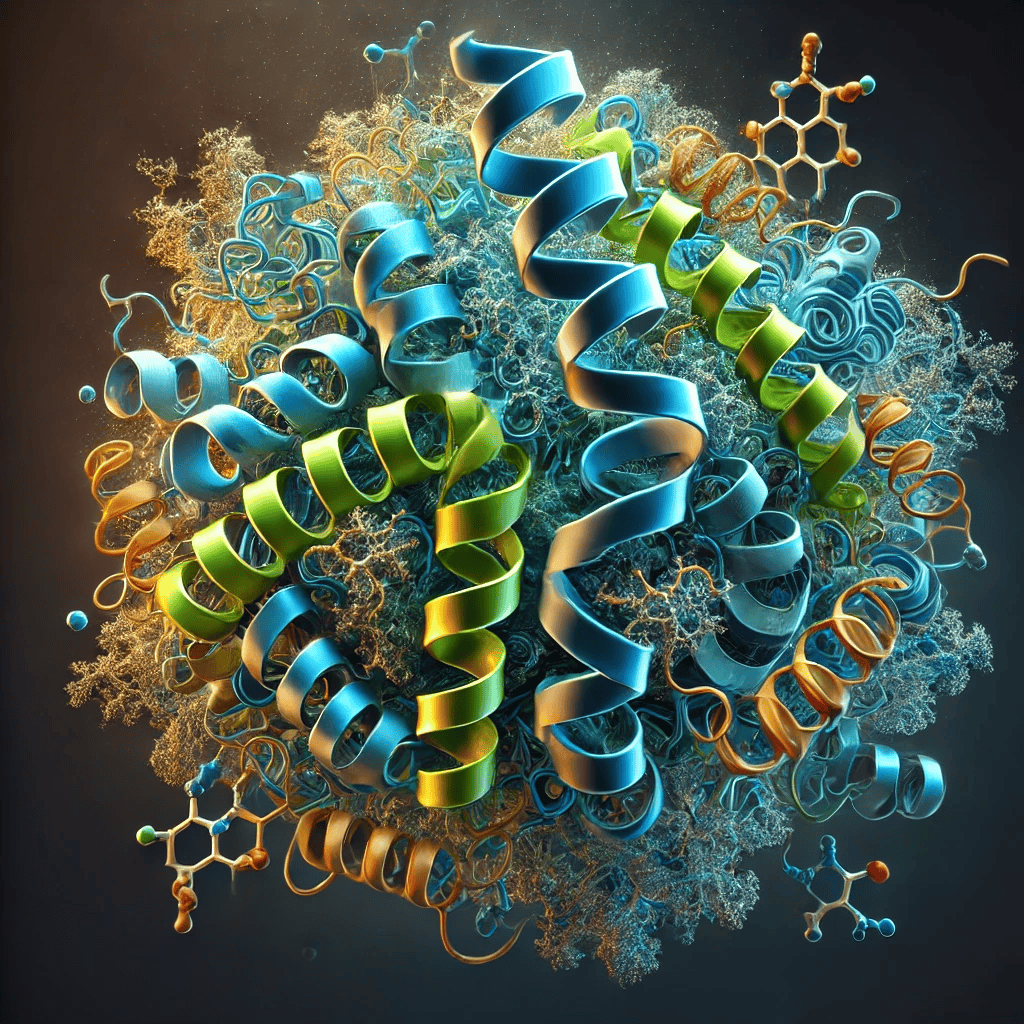
\includegraphics[width=0.8\textwidth]{proteins.png}

    \caption{Proteins can take on exotic conformations}
\end{figure}

Perhaps most significantly, the study of protein states through ECC's framework reveals how information processing can remain grounded in physical transitions while achieving remarkable computational sophistication \cite{Oldfield2014}. Rather than requiring abstraction into symbolic representation, neural computation occurs through actual changes in molecular configuration that maintain direct connection to energy flows. This perspective challenges purely computational approaches to consciousness while suggesting new directions for developing artificial systems capable of supporting conscious-like processing.

The implications extend beyond neuroscience to fundamental questions about the nature of information processing in biological systems \cite{Davis2018}. The remarkable sophistication of protein state dynamics demonstrates how evolution has refined molecular mechanisms to support both stable conscious states and flexible adaptation to changing conditions. This deeper appreciation of molecular complexity proves essential for any complete theory of consciousness and suggests new approaches to treating disorders of conscious processing.

The relationship between protein states and neural energetics reveals fundamental principles about biological computation \cite{Erickson2009}. The precise organization of conformational landscapes enables sophisticated information processing while maintaining direct connection to physical energy flows. This grounding in molecular dynamics helps explain how conscious systems achieve both stability and flexibility through carefully orchestrated patterns of state transitions \cite{Royer2006}.

Moving beyond individual proteins to examine direct cellular coupling, we must now consider how gap junctions enable coherent state maintenance across neural tissues. These specialized channels, composed of connexin proteins, create electrical synapses that allow for rapid, bidirectional communication between cells, proving essential for maintaining the coherent energy states necessary for conscious processing.

\section{Gap Junctions}

While individual protein states provide a basis for information encoding, gap junctions create direct cytoplasmic continuity between cells, enabling a fundamentally different form of information sharing and energy coupling. These specialized protein channels, composed of connexin proteins, form electrical synapses that allow for rapid, bidirectional communication between cells \cite{Giaume1996}. Unlike chemical synapses that rely on neurotransmitter release and receptor activation, gap junctions provide immediate electrical and metabolic coupling between connected cells.

The importance of gap junctions in neural processing extends far beyond simple electrical coupling. These channels enable the formation of functional syncytia - networks of coupled cells that can share states and coordinate their activities with minimal delay \cite{Bennett2004}. In neuronal networks, gap junctions prove particularly crucial for synchronizing populations of inhibitory interneurons, enabling precise temporal control over circuit activity. This rapid synchronization helps establish the coherent patterns of neural activity necessary for conscious processing.

Within glial networks, gap junctions take on even greater significance \cite{Dermietzel2013}. Astrocytes connected through these channels form extensive syncytial networks that can coordinate both metabolic support and information processing across substantial volumes of neural tissue. These networks enable sophisticated distribution of resources while maintaining stable background conditions for neural activity. The resulting patterns of cellular coupling provide essential mechanisms for supporting coherent conscious states.

The electrical properties of gap junctions demonstrate remarkable sophistication in their contribution to neural processing \cite{Connors2004}. These channels create low-resistance pathways between cells that enable rapid signal propagation while maintaining distinct functional domains. The voltage-dependent gating of gap junctions provides mechanisms for regulating cellular coupling based on local activity patterns. This dynamic regulation helps establish domains of coordinated activity that can maintain coherent states while adapting to changing conditions.

The molecular diversity of connexin proteins enables precise control over gap junction properties across different neural populations \cite{Willecke2002}. Various connexin subtypes create channels with distinct conductance properties and regulatory sensitivities, allowing for sophisticated modulation of cellular coupling. This molecular specialization enables neural tissues to maintain appropriate patterns of electrical and metabolic coupling while supporting diverse forms of information processing.

The regulation of gap junction coupling demonstrates sophisticated mechanisms for controlling cellular communication \cite{Nagy2018}. Conductance through these channels responds dynamically to various cellular signals, including voltage differences between cells, changes in pH and calcium levels, and modulation by phosphorylation states. This multilayered regulation enables precise control over cellular coupling while maintaining network stability.

The relationship between gap junctions and metabolic coordination reveals another crucial aspect of their function in conscious processing \cite{Hormuzdi2004}. These channels enable direct sharing of small molecules and metabolites between coupled cells, creating efficient pathways for distributing resources across neural tissues. This metabolic coupling helps maintain stable energy states while supporting dynamic patterns of neural activity. The coordination of cellular metabolism through gap junctions provides fundamental mechanisms for sustaining conscious processing.

Gap junctions play a particularly important role in establishing what might be termed coherence domains within neural tissue - regions where cells can maintain synchronized states through direct coupling \cite{Pannasch2013}. These domains emerge from the precise organization of gap junction connectivity, creating structured patterns of cellular communication that support conscious processing. The resulting network architecture enables both local coordination and broader patterns of coherent activity across neural populations.

The interaction between gap junctions and chemical synapses reveals sophisticated principles of neural organization \cite{Pereda2014}. Rather than operating independently, these different forms of cellular communication work together to create complex patterns of network activity. Gap junctions provide rapid synchronization and state sharing, while chemical synapses enable more nuanced control over information flow. This dual system of communication proves essential for maintaining coherent conscious states while enabling flexible neural computation.

The role of gap junctions in development and plasticity demonstrates their importance beyond immediate cellular coupling \cite{Nadarajah1996}. These channels influence how neural circuits form and modify their connectivity patterns, shaping both cellular differentiation and circuit refinement. The resulting patterns of gap junction connectivity reflect both genetic programming and activity-dependent modification. This developmental regulation helps establish the specific network architectures necessary for conscious processing.

The biophysical properties of gap junctions create unique opportunities for information processing \cite{Palacios-Prado2009}. The direct electrical coupling between cells enables forms of computation that would be impossible through chemical synapses alone. This specialized signaling capability proves particularly important for coordinating rapid responses across neural populations and maintaining coherent activity patterns.

The integration of gap junctional coupling with broader patterns of neural activity reveals fundamental principles about how conscious processing emerges from cellular interactions \cite{Nielsen2012}. Through their ability to create direct cellular coupling while maintaining dynamic regulation, gap junctions help establish the conditions necessary for consciousness. The resulting balance between rapid communication and controlled isolation enables neural systems to maintain coherent states while supporting complex information processing.

Perhaps most significantly, gap junctions demonstrate how biological systems achieve sophisticated coordination through physical mechanisms rather than abstract computation \cite{Bennett2004}. The direct sharing of electrical and metabolic states through these channels creates forms of cellular coupling that cannot be reduced to digital information processing. This understanding suggests new approaches to both studying consciousness and developing therapeutic interventions for neurological disorders.

The functional diversity of gap junction coupling across different neural populations reveals fundamental organizing principles of conscious processing \cite{Connors2004}. Different cell types and brain regions utilize distinct patterns of gap junction connectivity to achieve specific computational goals while maintaining broader network coherence. This architectural specialization demonstrates how biological systems can achieve both local specificity and global integration through direct cellular coupling.

The implications extend beyond neuroscience to fundamental questions about how biological systems maintain coherent states across multiple scales of organization \cite{Giaume1996}. The remarkable sophistication of gap junction networks demonstrates how evolution has refined cellular coupling mechanisms to support both stable conscious states and flexible adaptation to changing conditions. This deeper appreciation of biological connectivity proves essential for any complete theory of consciousness \cite{Hormuzdi2004}.

Moving beyond cellular networks, we must now examine how the cytoskeleton and its dynamic properties contribute to maintaining coherent conscious states. While previous theories have emphasized quantum effects in microtubules, the classical role of the cytoskeleton in organizing cellular energy dynamics and information processing provides crucial mechanisms for implementing ECC's principles.

\section{Cytoskeleton and Microtubules}

The cytoskeleton and microtubules represent crucial cellular infrastructure for maintaining coherent energy states in neural systems. While previous theories, particularly Penrose and Hameroff's Orchestrated Objective Reduction (Orch OR), emphasized quantum effects in microtubules, ECC focuses on their classical role in organizing cellular energy dynamics and information processing \cite{Fletcher2010}.

Microtubules form dynamic networks that serve multiple essential functions in maintaining conscious states \cite{Baas2011}. Their highly organized structure creates physical pathways for distributing energy and information throughout neurons and glial cells. This architectural role proves particularly significant in establishing and maintaining patterns of energetic coherence across cellular compartments. The precise spacing and orientation of microtubules shapes both local energy flows and broader field effects that contribute to conscious processing \cite{Conde2009}.

The dynamic instability of microtubules - their capacity to rapidly assemble and disassemble - provides a sophisticated mechanism for cellular adaptation to changing energy demands \cite{Howard2003}. This property enables neurons to reorganize their internal structure in response to activity patterns while maintaining overall coherence. Rather than representing noise or inefficiency, this dynamic reorganization allows cells to optimize their energy distribution networks in real-time \cite{Kapitein2015}.

Motor proteins moving along microtubules implement crucial aspects of cellular information processing through mechanical work \cite{Kueh2009}. These molecular motors transport organelles, vesicles, and other cellular components to specific locations, creating and maintaining the physical organization necessary for coherent energy states. The coordinated action of multiple motor proteins establishes complex patterns of energy flow that support conscious processing \cite{Kirschner1986}.

The interaction between microtubules and the cell membrane proves particularly significant for consciousness \cite{Wittmann2001}. Microtubules help organize membrane proteins and ion channels, influencing both local electrical properties and broader patterns of field coherence. This cytoskeletal-membrane coupling enables sophisticated regulation of energy flows between cellular compartments while maintaining stable conscious states.

Beyond their structural role, microtubules participate directly in cellular information processing through their effects on ion flows and electrical fields \cite{Dent2014}. Their hollow core structure and unique electrical properties influence how charge distributions evolve within cells. This contribution to cellular electrical properties helps establish the specific patterns of energetic coherence that ECC identifies as crucial for conscious processing.

The cytoskeleton's role in synaptic plasticity further demonstrates its importance for consciousness \cite{Kapitein2015}. Through activity-dependent reorganization, the cytoskeletal network enables both rapid synaptic modifications and longer-term structural changes that support learning and memory. This capacity for controlled reorganization while maintaining coherent function proves essential for consciousness's combination of stability and adaptability.

Understanding the cytoskeleton and microtubules through ECC's framework suggests new approaches to investigating consciousness \cite{Nogales2000}. Rather than searching for quantum effects, research might productively focus on how these cellular structures enable and constrain patterns of energetic coherence across multiple scales of neural organization. This classical yet sophisticated role may prove more fundamental to consciousness than previously recognized.

The cytoskeleton's influence on cellular energy dynamics extends beyond structural support through its role in signal transduction and mechanotransduction \cite{Fletcher2010}. Actin filaments, intermediate filaments, and microtubules together create a sophisticated tensegrity structure that enables cells to sense and respond to mechanical forces while maintaining coherent energy states. This mechanical sensitivity proves crucial for how neural tissues integrate information across multiple physical modalities.

The relationship between cytoskeletal organization and astrocytic function deserves particular attention \cite{Sanchez-Huertas2016}. Astrocytes maintain extensive cytoskeletal networks that enable them to coordinate both metabolic support and information processing across substantial volumes of neural tissue. Their cytoskeletal architecture supports the formation and maintenance of the syncytial networks that ECC identifies as crucial for conscious integration.

Microtubule-associated proteins (MAPs) play essential roles in regulating cytoskeletal dynamics and cellular organization \cite{Roll-Mecak2020}. These proteins modify how microtubules interact with other cellular components, enabling sophisticated control over energy distribution and information flow. The rich variety of MAPs expressed in neural tissues creates a molecular alphabet - a diverse repertoire of possible states that supports complex information processing while maintaining energetic coherence.

The cytoskeleton's role in neural development illuminates how conscious processing requires specific patterns of cellular organization \cite{Stiess2011}. During neuronal differentiation and circuit formation, the cytoskeleton guides axon pathfinding, dendritic arborization, and synaptic organization. These developmental processes establish the physical architecture necessary for maintaining coherent energy states across neural networks.

Intracellular transport along cytoskeletal networks proves particularly crucial for maintaining conscious states \cite{Vallee2006}. Coordinated movement of mitochondria, synaptic vesicles, and other cellular components allows neurons to match energy supply with local demand while maintaining coherent function. This sophisticated logistics system, operating through molecular motors and cytoskeletal tracks, supports the specific patterns of energy distribution that consciousness requires.

The interaction between cytoskeletal networks and ion channels demonstrates another crucial aspect of cellular information processing \cite{Conde2009}. Microtubules and actin filaments influence both the distribution and function of ion channels in cellular membranes. This organization of ion channels shapes local electrical properties while contributing to broader patterns of field coherence across neural tissues. The resulting integration of mechanical and electrical signaling enables sophisticated forms of information processing that transcend simple neural computation.

These cytoskeletal mechanisms take on new significance when viewed through ECC's emphasis on energy dynamics rather than quantum effects \cite{Baas2011}. While preserving insights about cytoskeletal importance from previous theories, this classical perspective grounds consciousness more firmly in well-understood biological mechanisms while suggesting new directions for research and therapeutic intervention.

The multifaceted roles of the cytoskeleton in maintaining cellular coherence exemplify how biological systems achieve sophisticated information processing through physical organization rather than abstract computation \cite{Fletcher2010}. From structural support to signal integration, from energy distribution to information processing, the cytoskeletal network demonstrates how consciousness emerges from precisely organized cellular dynamics operating across multiple scales.

Understanding the cytoskeleton through ECC's framework suggests new therapeutic approaches for disorders of consciousness. Rather than targeting neurotransmitter systems alone, interventions might focus on supporting or modifying cytoskeletal organization to restore patterns of energetic coherence. This perspective offers fresh insights for treating conditions ranging from traumatic brain injury to neurodegenerative diseases.

The cytoskeleton thus emerges not merely as cellular scaffolding but as a fundamental substrate for the energetic coherence that consciousness requires. Its sophisticated organization and dynamic properties enable biological systems to achieve remarkable information processing capabilities while maintaining the specific patterns of energy flow that support conscious experience.

\newpage
\section{References}
\printbibliography[title={},heading=subbibliography]
%\printbibliography[title={References: Biological Implementation}]
\end{refsection}